\documentclass[11pt, a4paper]{article}
\usepackage{graphicx}
\usepackage{amsmath, bm}
\usepackage{natbib}
\usepackage[utf8]{inputenc}    
\usepackage{natbib}
\usepackage[usenames,dvipsnames]{xcolor}
\usepackage[left=2cm,right=2cm,top=2cm,bottom=2cm]{geometry}
\usepackage{hyperref}
\usepackage[outdir=./]{epstopdf}
\usepackage{lscape}
\usepackage{float}  % PUT FIGURE HERE
\usepackage{multirow}
\usepackage{booktabs} % Create TABS
%\usepackage{array,arydshln}  % CREATE DASH LINE
\title{Identification of stably expressed genes from Arabidopsis RNA-Seq data}
\date{} % Today's date or a custom date



\hypersetup{
    colorlinks,
    citecolor=blue,
    filecolor=blue,
    linkcolor=blue,
    urlcolor=blue
}

\begin{document}

Our main points include: 
\begin{enumerate}
    \item using multiple (a larger number of) public-available existing/past data sets, 
	\begin{enumerate}
	    \item
		using multiple data sets 
		\begin{enumerate}
		    \item
			as compared to using a single data set: a numerical
			measure of expression stability (typically, measures
			of certain aspects of RNA-Seq count variation) can be
			more reliably estimated by using more data sets (???)
		    \item
			(leaf) learn variance components (see GLMM)
		    \item
			(leaf) using top 1000 identified genes for
			normalization
		    \item
			(discussion) use as prior information in Bayesian analysis or
			use the  set for quality control/vanity check purpose
		\end{enumerate}
	    \item
		(caveat) genes that are stable under a range of conditions
		might not be the most stable under a particular condition
		(under a single experiment).
		\begin{enumerate}
		    \item
			(leaf) identify different reference sets for different tissue
			types
		\end{enumerate}

	    \item Subtle points on interpretability and comparability (??? do
		we need some toy examples)

		\begin{enumerate}
		    \item
			using an explicit reference set: improve interpretability
		    \item
			using a common reference set (when comparing two or more studies): improve comparability
		\end{enumerate}
	\end{enumerate}

    \item
	using a numerical measure of stability
	\begin{enumerate}
	    \item
		(leaf) stability of house-keeping genes (HKGs)
	    \item
		(leaf) different numerical measures (geNorm, normFinder)
	    \item
		(leaf) different data sources (microarray and RNA-Seq)
	    \item
		(discussion) numerical measure of stability vs biological
		stability 
	\end{enumerate}


    \item
	Validate the stably expressed genes that we find? (no leaf yet) 
	\begin{enumerate}
	    \item
		biological function (online database) 
	    \item
		(GO analysis)
	\end{enumerate}

    \item
	Future, use our methods and leaf (stable set, rankings, variance
	components) in real studies.
\end{enumerate}

\newpage
\maketitle

\section*{Abstract}
We examined RNA-Seq data on 209 biological samples from 23 different
experiments carried out by different labs and identified genes that are stably
expressed across biological samples, experiment conditions, and labs. We fit a
random-effect model to the read counts for each gene and decompose the total
variance to into between-sample, between-treatment and between-experiment variance
components. Identifying stably expressed genes is useful for count
normalization and differential expression analysis. The variance component analysis is a first step towards
understanding the sources and nature of the RNA-Seq count variation.


\section{Introduction}\label{section:Introduction}

\textbf{(overview)}
RNA sequencing (RNA-Seq) has become the technology of choice for transcriptome
profiling over the last few years. The exponential growth in RNA-Seq study has
accumulated a large amount of Arabidopsis data under a variety of
experimental/enviromental conditions.  It is only natural to begin exploring
how the large amount of existing data sets can help the analysis of future
data.  In this paper, we discuss identifying stably expressed genes from
multiple existing RNA-Seq data sets based on a numerical measure of stability.
We envision that such identified stably expressed genes can be used as a
reference set or prior information for count normalization and differential
expression (DE) analysis of future RNA-Seq data sets obtained from similar or
comparable experiments.  We also fit a random-effect model to the read counts
for each gene and decompose the total variance to into between-sample,
between-treatment and between-experiment variance components. The variance component
analysis is a first step towards understanding the sources and nature of the
RNA-Seq count variation.  To illustrate our methods, we examined RNA-Seq data
on 209 Arabidopsis  samples from 23 different experiments carried out by
different labs and identified genes that are stably expressed across
biological samples, experiment conditions, and labs.  

A reference set of stably-expressed genes will be useful for count
normalization.  A key task of RNA-Seq analysis is to detect DE genes under
various experimental or environmental conditions. Count normalization is
needed for adjusting differences in sequencing depths or library sizes (total
numbers of mapped reads for each biological sample) due to chance variation in
sample preparation.  In DE analysis, gene expression levels are often
estimated from relative read frequencies. For this reason, normalization is
also needed to account for the apparent reduction or increase in relative read
frequencies of non-differentially expressing genes simply to accommodate the
increased or decreased relative read frequencies of truly differentially
expressing genes.  Many existing normalization methods, such as the trimmed
mean of M-values normalization method (TMM) \citep{robinson2010scaling} and
DESeq normalization \citep{anders2010differential}, will  assume that the
majority of the genes are not DE within an experiment and examine the sample
distribution of the fold changes between samples.
% There are two obvious
% difficulties when using such a normalization method: 1) There is great
% uncertainty in observed fold changes.  
% is typical available sample size in any single experiment can be too small
% for us to reliably estimate true fold changes.  
If the experiment condition can affect expression levels of more than half of
the genes, many of the existing normalization methods may be unreliable
(\cite{loven2012revisiting}, \cite{wu2013use}).  This difficulty can be
alleviated if one could identify a set of stably expressed genes whose
expression levels are known or expected to not vary much under different
experimental conditions. Our idea is to identify such a reference set based on
a large number of existing data sets.

Our basic intuition is that a numerical quantification of expression
stability---which typically measures certain aspects of RNA-Seq count
variation---can be more reliably estimated by using more data sets.  There is,
however, a caveat to this idea: as pointed out by \cite{hruz2011refgenes},
universally stably expressed genes may not exist and a subset of stably
expressed genes from a specific biological context may have less variability
than those identified across varying tissues and conditions.  Many studies
have shown that stably expressed genes are subject to change from one
experiment to another, either due to varying experimental protocols, or due to
different organs of a given species (\cite{reid2006optimized},
\cite{hong2010identification}).  The top 100 stably expressed genes in developmental series of 
\cite{czechowski2005genome} shared only 3 genes with top 50 stably expressed
genes identified from Arabidopsis seed samples by \cite{dekkers2012identification}.  In this
study, we try to balance the generality and specificity by identify different
reference gene sets for different tissue types of Arabidopsis. 

We can also think that when a normalization method is applied to a single data
set, it effectively specifies an implicit reference set of stably expressed
genes (those genes that has least variation after normalization). We can think
this as using an internal reference set. In contrast, what we are proposing is
that one can also identify an external reference set by looking at past data
sets. The internal and external reference sets will provide different contexts
for the DE analysis: in other words, one can choose to answer different
scientific questions by using different reference sets. In any case, we
advocate  making the reference set explicit during a DE analysis and using a
common reference set when analyzing multiple datasets. We will further discuss
these points in the Discussion section (REF).


In this paper, we identify stably expressed genes from RNA-Seq data sets based
on a numerical measure---the sum of three random components estimated from a
mixed-effect model.  We want to clarify that there is a distinction between
numerical stability and biological stability---often times, we may not
understand the biological functions of genes with numerically stable
expression measures.  From an operational point of view, however, numerical
stability is more tractable.  In pre-genomic era, the so-called "house-keeping
genes" are often considered as candidates of reference genes for
normalization (\cite{bustin2002quantification},
\cite{andersen2004normalization}). house-keeping
genes are typically constitutive genes that
maintain basic cellular function, and therefore are expected to express at
relatively constant levels in non-pathological situations.  However, many
studies have shown that house-keeping
genes are not necessarily stably expressed according to
numerical measures (a review can be found in \cite{huggett2005real} and
reference therein).  For example, in the microarray analysis of the model
plant \textit{Arabidopsis thaliana} (Arabidopsis), \cite{czechowski2005genome}
showed that traditional house-keeping
genes such as ACT2, TUB6, EF-1$\alpha$ are not stably
expressed, and thus not good reference genes for normalization.  Spike-in
genes have also been considered as reference genes for normalization, but
\cite{risso2014nat} showed that spike-in genes are not necessarily stably
expressed according numerical measures either.  
% HKGs or spike-in genes thus cannot be taken as granted as stably expressed
% genes for count normalization purpose.  and careful evaluation should be
% performed when they are being used in normalization. (??? simplify, make
% concise)
%\textbf{Numerically finding stably expressed genes.}
% Why would we bother to study them under RNA-Seq since there are related
% works in microarray} (some sentense are needed to connect the two
% paragraphs)
For microarray data, there are many efforts to numerically find stably
expressed genes by quantifying the variation of measured expression levels
across a large number of microarray data sets.  For example,
\cite{czechowski2005genome} measured the expression stability of each gene
using the coefficient of variation (CV). Genes with lower CVs are considered
as more stably expressed.  By investigating 721 arrays under 323 conditions
throughout development, \cite{czechowski2005genome} suggested stably expressed
(reference) genes under different experimental conditions for Arabidopsis.
% find stably expressed genes based on 526. 
%and  validated a subset of most stably expressed genes they identified.
%Similar studies were carried out for Arabidopsis seed
\cite{stamova2009identification},  \citet{dekkers2012identification}, \citet{gur2009identification}, and
 \citet{frericks2008toolbox} screened a large number of microarray data sets
 to identify stably expressed genes in human blood, Arabidopsis seed, breast tumor tissues,
 and mice respectively.
% Similar studies were carried out for Arabidopsis seed
% \citep{dekkers2012identification}, breast tumor
% tissues\citep{gur2009identification}, mouse (universal)
% \citep{frericks2008toolbox} and so on.  
Validation experiments (\cite{czechowski2005genome},
\cite{dekkers2012identification}, \cite{huggett2005real},
\cite{stamova2009identification}) showed that these genes are more stably
expressed than traditional house-keeping genes.  




The rest of the paper organized as follows: in \ref{section:{section:countNormalization}}, we describe the data collection and processing steps. In \ref{section:countNormalization}, we give a brief review normalization methods, which is needed for fitting a generalized linear mixed model (GLMM) \citep{mccullagh1989generalized} in our method presented in Section \ref{subsection:OurMethod}. We compare the stably expressed genes with previous studies in \ref{section:stablyExpressedGene} and \ref{section:CompareStablyExpressedGene}, and discuss expression stability in terms of different stability measures and of different data sources in section \ref{section:stabilityMeasure}. We present variance components in \ref{Section:varianceComp} and recommend stably expressed genes for normalization in \ref{Section:commonReference}.

\section{Methods} \label{section:Methods}
(Overview) In this section, we discussed our method of identifying stably expressed genes. In 1, we described how the Arabidopsis RNA-Seq data sets are collected and cleaned. In 2, we briefly discussed count normalization method, which is needed for fitting our GLMM model. Our main method is presented in 3, where we fit a GLMM to each gene and estimate three variance components: the \textit{between-sample}, \textit{between-treatment} and \textit{between-experiment} variances.
 The \textit{total variance} is defined to be the expression stability measure associated with that gene. Genes with smaller total variance are considered to be more stably expressed. 



\subsection{Data collection}\label{section:DataCollection}
The \textit{Gene Expression Omnibus} (GEO) repository at \textit{National Center for Biotechnology Information} ( NCBI, \url{http://www.ncbi.nlm.nih.gov/}) contains a large number of RNA-Seq experiments. The RNA-Seq read count data were either processed by different aligners or not directly available at NCBI. For this reason, we developed a pipeline based on the Subread aligner \citep{liao2013subread} to process raw FASTQ data into read counts. The pipeline, based on \verb"Rsubread" (version 1.16.2), is summarized as follows: Step 1, \textit{Sequence Read Archive} (SRA) format files of Arabidopsis samples were retrieved from GEO repository, and then converted to
FASTQ files using NCBI SRA Toolkit (\url{http://www.ncbi.nlm.nih.gov/Traces/sra/sra.cgi?cmd=show&f=software&m=software&s=software}, version 2.3.5-2). Step 2, the Arabidopsis reference genome was downloaded through the\textit{ Ensembl plants FTP server}
(\url{http://plants.ensembl.org/info/data/ftp/index. html}). As suggested by
\cite{anders2013count}, "FASTA(DNA)" link was chosen because samples were aligned 
to the genome. The index was built subsequently for read mapping by \verb|buildindex()|.  Step 3, short reads were mapped to the reference genome by \verb"align()" and read counts
were obtained by \verb"featureCounts()". Default options for the two functions were used except that
the annotation file is set to be \verb"Arabidopsis_thaliana.TAIR10.22.gtf", which is desired for matching the short reads to Arabidopsis genes. % The multi-mapping or multi-overlapping reads were not counted (included in the default option).


  (\textbf{Selecting experiments}) For this study, our attention is restricted to experiments satisfying all the following conditions:  1. Ecotype = "Columbia" ( as a result, we might only choose the Columbia samples when the experiment is done to compare Columbia with other ecotypes.); 2. Library strategy= "RNA-Seq"; 3. Library Source = "transcriptomic"; 4. Library selection= "cDNA"; 5. Library layout = "Single End"; 6. there are at least 2 biological replicates for each treatment. We screened all the Arabidopsis experiments available at NCBI up to May 31, 2015, and processed a total of 49 data sets. Each data set is named by its accession number. 
    

  
   
   
  (\textbf{Selecting samples}) \cite{czechowski2005genome}, \cite{hruz2011refgenes}, and
   \cite{dekkers2012identification} show that transcriptomes vary across different tissue types and development stages. For this reason, we separated the data sets into three groups: the seedling group where only Arabidopsis seedling are included, the leaf group where only Arabidopsis leaves are included, and the multiple-tissue group where different tissue types are included. Within each group, we pre-screened experiments by treatment structures and data quality: 1. If there are repeated measurements over time, we chose only one time period (this includes GSE39463 and GSE43865); 2. We chose experiments with \textit{initial DESeq normalization factors} (discussed in \ref{section:countNormalization}) ranging from 0.70 to 1.30: that is, the experiment is retained only when minimun of normalization factors is greater than 0.7 and maximun of normlization factors is less than 1.3. 
   
    Eventually, we obtained 23 data sets (with 209 biological samples): 10 experiments (70 samples) for seedling group, 5 experiments (60 samples) for leaf group and 8 experiments (79 samples) for multiple-tissue (shoot apical,  root tip, primary root, inflorescences and siliques, hypocotyl, flower, carpels, aerial tissue) group. Samples from different experiments were merged by their unique gene IDs, and then stored as read count matrices. A brief description of the data sets can be found in Table (REF) supplementary material. More details for each experiment are also accessible at NCBI via the unique accession number provided in Table (REF).
   
   
	 (Selecting genes) Prior to analysis, we removed genes with low overall counts as suggested by \cite{anders2013count}. Filtering lowly-expressed genes is helpful not only because such genes provide little information about expression level,  but also because they will cause convergence failure to our model. In practice, convergence issue can be avoided by removing genes with overall mean count less than 3. Table \ref{table:TableSet3} summarizes the three groups after removing lowly-expressed genes.
   
   \begin{table}[h]
   	\centering
   	\caption[3.2]{data set summary}
   	\begin{tabular}{lrrrr} \hline
   		Group & \# of experiments & \# of treatments  & \# of biological samples & \# of genes \\ \hline
   		Seedling &10 & 31 &70  &24379  \\
   		Leaf &5 & 28 & 60 &20967  \\
   		Multiple-tissue &8 &35  &79  & 23666\\ \hline
   		 \label{table:TableSet3}
   	\end{tabular}
   \end{table}
   

%\textbf{Moved from introduction part, or better to put it in discussion part?}
%\cite{czechowski2005genome} and \cite{dekkers2012identification} adopted similar approach for statistical analysis for identifying stably expressed genes, and both used Arabidopsis microarray data. Briefly, for each gene the mean expression and the standard deviation (SD) over all biological samples are calculated, and the coefficients of variation (CV), which is the ratio of SD to mean expression, are obtained. Genes with lower CVs are expected to be more stably expressed. This simple approach, however, does not provide us any information about possible sources, except the amounts,  of variation.  \textbf{}\\ 

\subsection{Count normalization}\label{section:countNormalization}

Many existing normalization methods, such as the trimmed mean of M-values normalization method (TMM) \citep{robinson2010scaling} and DESeq normalization \citep{anders2010differential}, assume that the majority of the genes are not DE within an experiment. Effectively, these methods use genes with relatively small observed fold changes under a single experiment as a reference gene set in normalization. We choose DESeq \citep{anders2010differential} as our normalization method in this paper. Briefly, let $y_{ij}$ denote the read count for $i$th gene and $j$th sample, then a pseudo-reference sample is created, with gene $i$th expression value defined as the geometric mean of the same gene over all real samples, 
\[ z_i = (\prod_{j=1}^ny_{ij})^{1/n},  i=1, \ldots, m \]
 The normalization factor for sample $j$ is then calculated as the median of the fold-changes between sample $j$ and pseudo-reference sample over all genes
  \[N_j = \text{median}(y_{1j}/z_1, \ldots, y_{nj}/z_n)\]
  We used all the genes to calculate initial normalization factors, which served as an \textit{offset} to estimate the three variance components in GLMM of equation \ref{eq:GLMM} of Section \ref{subsection:OurMethod}. The total variance was used to rank the genes (discussed in \ref{subsection:OurMethod}), and top 1000 genes were used as reference genes to calculate the new normalization factors in our analysis herein. 

\subsection{Poisson log-linear mixed-effects regression model}\label{subsection:OurMethod} 
% (Each individual count is model as a Poisson distribution. The count mean is
% modeled through a log-linear mixed-effects regression model.)


Let $Y_{ijkl}$ denote the read count for $i$th gene
in $j$th observational unit of $k$th treatment group in $l$th experiment
and index $i$ is suppressed herein since only one gene is evaluated at a time
by GLMM of  equation \ref{eq:GLMM}. We assume that each read count follow a Poisson
distribution,  
\[Y_{jkl}\sim \text{Poisson}(\mu_{jkl}).\] 
We use a log-linear Poisson regression model to capture 
the variation of $\mu_{jkl}$ across samples and experimental conditions (treatments,
organs, sequencing platforms etc.),
\begin{equation}\label{eq:GLMM}
    \log( \mu_{jkl}) = \xi + \log(R_{jkl}N_{jkl})+ \alpha_l + \beta_{k(l)} + \epsilon_{jkl} 
\end{equation}
where $\alpha$s are experiment effects,  $\beta$s are treatment effects
nested in experiments, and $\epsilon$s are the effects for biological samples. 
$R_{jkl}$ is the library size (column sum), and the $N_{jkl}$ is the normalization factors discussed in
subsection (\ref{section:countNormalization}). The product term $R_{jkl}N_{jkl}$ is called \textit{effective library size} in DE analysis. 

The between-experiment effect $\alpha$ in (\ref{eq:GLMM}) is treated as random for two considerations. First, we view the collected data sets as a random sample from the pool of all Arabidopsis RNA-Seq experiments. Second, we expect the results from this study to be generalizable to future experiments when it comes to stably expressed genes and variance component analysis.
We also consider the treatment effects $\beta$ as random 
in the sense that treatment in future experiments may be different from this study.

We assume that $\alpha$'s, $\beta$'s and $\epsilon$'s are mutually independent, and  
%   \[ \log( \mu_{ijk}) = \xi + \log(R_{ijk}N_{ijk})+ \alpha_k + \beta_{j(k)} + \epsilon_{ijk} \]
  \[\alpha_l\sim N(0, \sigma^2_{\text{experiment}}),\] 
  \[\beta_{k(l)}\sim N(0, \sigma^2_{\text{treatment}}),\]
   \[\epsilon_{jkl}\sim N(0, \sigma_{\text{sample}}^2).\]
$\sigma_{\text{sample}}^2$, $\sigma_{\text{treatment}}^2$, $\sigma_{\text{experiment}}^2$ are called \textit{variance-components}. They capture the
\textit{between-sample}, \textit{between-treatment} and \textit{between-experiment} variation
correspondingly. The between-sample variance plays a similar role as the over-dispersion, which represents extra-Poisson variation in read counts under a negative binomial model (\cite{anders2010differential},\cite{di2011nbp}).  The between-treatment term accounts for variations in treatment condition (e.g. genotype, growth medium). 
The between-experiment variation includes all other possible variations that are difficult to be separated statistically, for example, lab personnel and conditions, day light hours, age of the plants, temperature, sequencing platform, etc.

The stability measure of a given gene is defined by its total variance
 \begin{equation}\label{eq:totalVariance}
 \sigma^2 =\sigma_{\text{sample}}^2+ \sigma_{\text{treatment}}^2+ \sigma_{\text{experiment}}^2
 \end{equation}
For each gene, we obtain the estimated variance components $\hat\sigma_{\text{sample}}^2,  \hat\sigma_{\text{treatment}}^2,  \hat\sigma_{\text{experiment}}^2$ and the total variance $\hat\sigma^2$ from (\ref{eq:GLMM}).
We rank all the genes according to their $\hat\sigma^2$s. and consider highly ranked (top 1000) genes to be stably expressed. 

\subsection{Other stability measures}\label{subsection:OtherStabilityMeasure}
There are many other gene expression stability measures for microarray data, among which the $M$ value in \textit{geNorm} \citep{vandesompele2002accurate} and the $\rho$ value in \textit{NormFinder} \citep{andersen2004normalization} are popular. In geNorm, the relative variation $\text{SD}_{i, i_1}$ of genes $i$ to gene $i_1$ is calculated as the standard deviation of the log fold changes between the two genes, $\text{SD}_{i, i_1} = \text{standard deviation}(\log_2 \frac{y_{i1}}{y_{i_11}}, \ldots, \log_2 \frac{y_{im}}{y_{i_1m}})$ where $m$ is the total number of genes in the reference set; then the stability value $V_i$ for gene $i$ is the mean of pairwise variation between gene $i$ and the other $m-1$ genes, 
\begin{equation}\label{eq:vvalue}
V_i = \sum_{i_1 \neq i}\text{SD}_{i, i_1}/m
\end{equation}
Stably expressed genes are expected to have low $M$ values. NormFinder uses a linear mixed model to estimate the between-group and within-group variations from expression values of microarray data, and then combines the two variations by a Bayesian formulation. For a future experiment, the stability of a given gene is defined as the its absolute value of posterior mean plus its standard prediction deviation. Alternatively, \cite{czechowski2005genome} and \cite{dekkers2012identification} use CV (standard deviation/mean) to measure expression stability, with smaller CV  corresponding to more stably expressed genes.
	
Stability measures differ in summarizing variation of gene expression profiles. The total variance ${\sigma}^2$ considers genes to be stably expressed when they have low ${\sigma}^2$ in the estimated log relative mean
counts; the $M$ value in geNorm identifies as stably
expressed those genes that are most similar to each other; and the CV measure
\citep{czechowski2005genome} tends to select highly expressed genes as stable
since those genes tend to have smaller dispersion \citep{hruz2011refgenes}. The idea GLMM (equation \ref{eq:GLMM}) is similar to the linear mixed model in NormFinder. However, NormFinder works for normally distributed expression data and requires a minimun of eight samples per treatment \citep{andersen2004normalization}, therefore it will not be discussed in this paper. %since the sample size is small (two or three samples per treatment) in a typical RNA-Seq experiment.



\section{Results} \label{section:Results}
In Section \ref{section:stablyExpressedGene}, we summarize stably expressed genes identified from three
different experiment groups and one emphasis is that stability is
context dependent. In Section \ref{section:CompareStablyExpressedGene}, we show that traditional housekeeping
genes are not necessarily stably expressed according to our numerical measure
and microarray data and RNA-Seq data will give different sets of stably
expressed genes.  In Section \ref{section:stabilityMeasure}, we further demonstrate that when using a
numerical measure to measure gene expression stability, the outcome will
depend on the specific numeric measure used.  These points should be
obvious/intuitive, but they are not often emphasized in practice. 
In Section \ref{Section:varianceComp}, we discuss variance component analysis. In Section
\ref{Section:commonReference}, we discussed how to use the identified stably expressed genes for count
normalization.

\subsection{Stably Expressed Genes}\label{section:stablyExpressedGene}
Using the total variance, $\sigma^2$, from the GLMM (see
equation \ref{eq:GLMM} in Section \ref{subsection:OurMethod}) as a
stability measure, we identified stably expressed genes in three groups of
experiments described/summarized in Section \ref{section:countNormalization}: the group of seedling
experiments, the group of leaf experiments, the group of experiments on
different tissue types (see Table \ref{table:TableSet3} for a summary).  (The
seedling group consists of 70 samples from 10 experiments on Arabidopsis
seedlings; the leaf group consists 60 samples from 5 experiments on
Arabidopsis leaf; and the multiple-tissue-type group consists 79 samples from
different 8 experiments on different tissues types.) As we mentioned in
Introduction, absolutely stably expressed genes may not exist.  Choosing
different external reference data sets allows us to identify the stably
expressed genes for different biological contexts.

% Method section \ref{section:{section:countNormalization}}: the group of seedling
% experiments, the group of leafexperiments, the group of experiments on
% different tissue types. The seedlinggroup consists of 70 samples from 10
% experiments on Arabidopsis seedlings; theleaf group consists 60 samples from 5
% experiments on Arabidopsis leaves; andmultiple-tissue-type group consists 79
% samples from different 8 experiments ondifferent tissues types.  
In Tables 1-3 (REF) in the online supplementary materials, we summarize the
top 1000 most stably expressed genes in each group.  In Figure \ref{cpm}, we
summarize the histograms of the mean Count Per Million (CPM) for the 1000
most stably expressed genes identified in each group. For each gene, the CPM
is computed as \[ \dfrac{ \text{count} \times 10^6 }{ \text{normalized library
size}} \] in each sample and the mean is computed over all samples.
 
\begin{figure}[] \begin{center}
    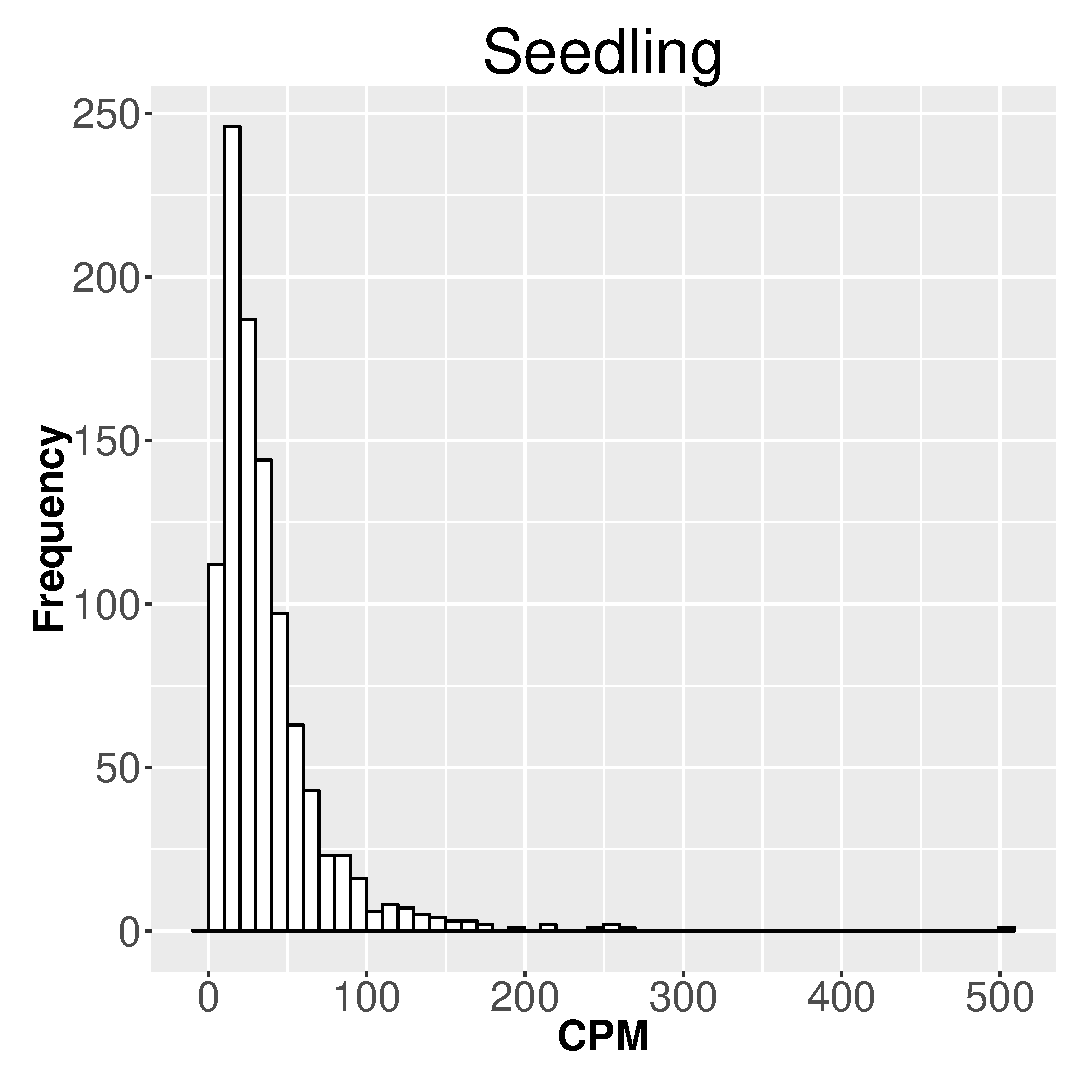
\includegraphics[width=5cm,height=4cm]{Figures/cpm_seedling.eps}
    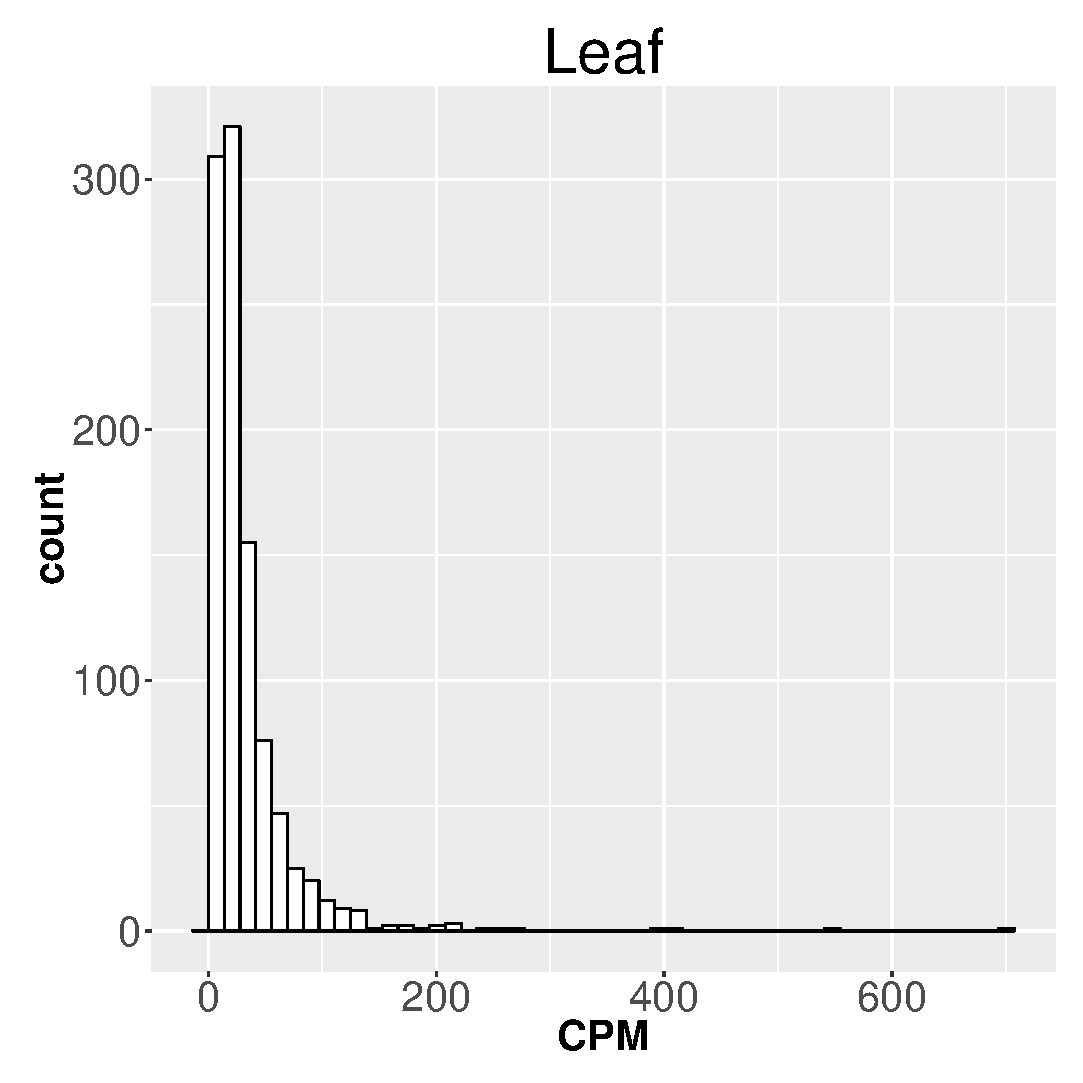
\includegraphics[width=5cm,height=4cm]{Figures/cpm_leaves.eps}
    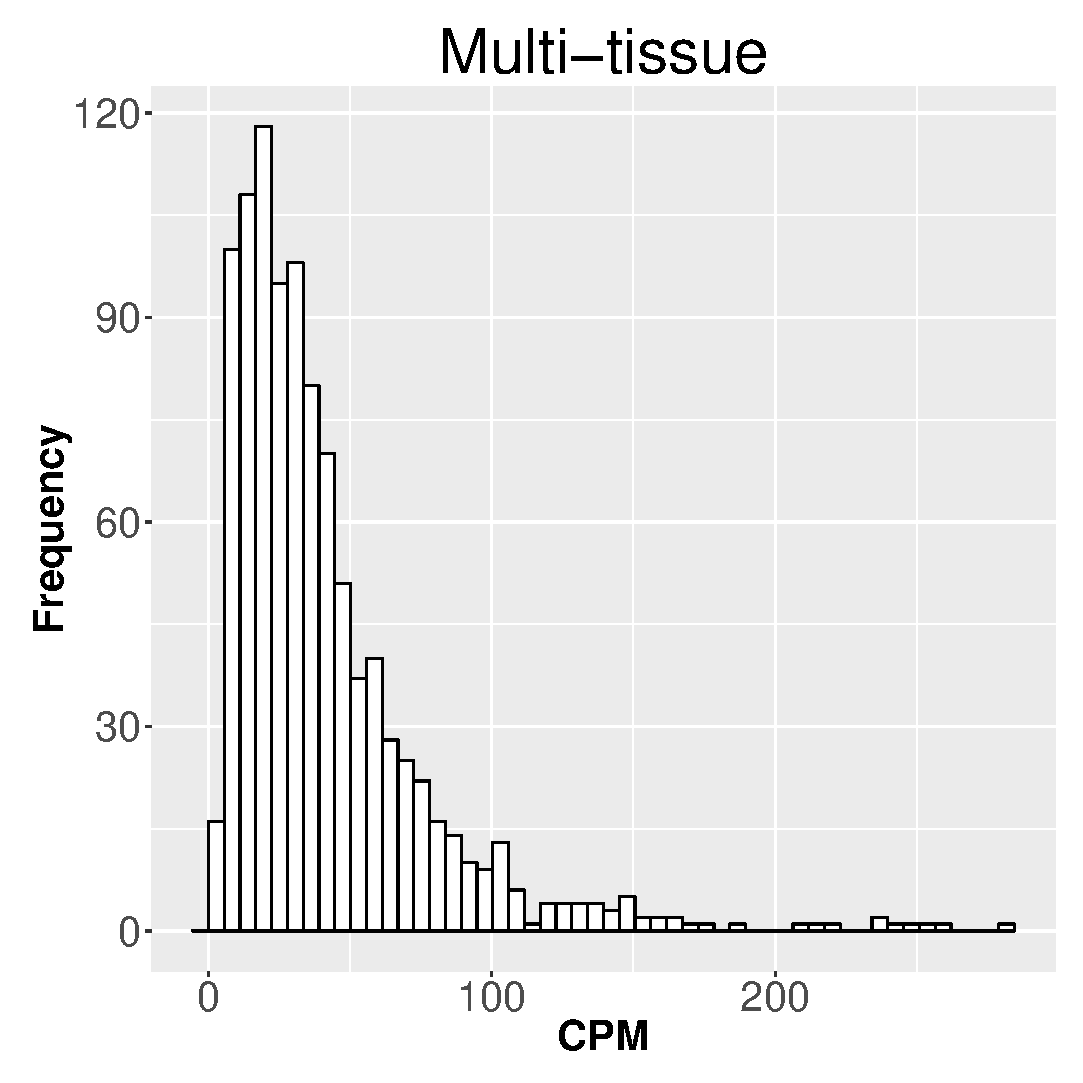
\includegraphics[width=5cm,height=4cm]{Figures/cpm_tissue.eps}
    \caption{{\small{\label{cpm} mean CPM for the top 1000 most stably
    expressed genes, seedling (left), leaf (middle) and multiple tissue
    (right) }}} \end{center} 
\end{figure} 

% The mean CPM  of top 1000 genes, each averaged across all samples, vary from
% 2.0 to 499.0 for seedling, from 0.2 to 693.4 for leaves, and 0.4 to 278.8,
% constituting a broad range of expression values.

Comparison of the lists of top 1000 genes in the three groups reveals that
they share 106 genes in common (see supplement material for detail).  These
genes are stably expressed under a wide range of experimental conditions
and in different tissue types, and thus may be worth further study.  In particular, one
gene, AT1G13320, was identified by \cite{hong2010identification} as a stably
expressed gene under all six but one experimental conditions he examined, and it is in
all ten but one list of top 500 stably expressed genes identified by
\cite{czechowski2005genome} for different experimental and experimental
conditions (the one exception being the set of diurnal series, ??? Jeff).
This gene is ranked 446 (top 1.8\%), 112 (top 0.5\%), 687 (top 2.9\%)
according to our stably measure in the three groups we examined.  (??? Is
there anything special about this gene? Jeff) This gene is a subunite of
protein phosphatase type 2A complex and involves in regulation of
phosphorylation and regulation of protein phosphatase type 2A activity. It has
been used as a reference gene in many papers (??? REF
\url{https://www.arabidopsis.org/servlets/TairObject?name=AT1G13320&type=locus}).  

\subsection{Comparison to house-keeping genes and stably expressed genes
identified from microarray data}\label{section:CompareStablyExpressedGene}
\cite{czechowski2005genome} discussed the expression stability of
house-keeping genes and showed that the house-keeping genes are not stably
expressed according to their numerical measure. In particular, they compared
the expression profiles of five traditional house-keeping genes (AT1G13440,
AT3G18780, AT4G05320, AT5G12250, AT5G60390) and five genes (AT1G13320,
AT5G59830, AT2G28390, AT4G33380 and AT4G34270) that they identified  as stably
expressed according to the CV measure from a developmental series of
microarray experiments (see Figure 1 of that paper).  
In Figure \ref{expressinlevel1}, we compare the expression profiles 
of these 10 genes from \cite{czechowski2005genome} to the expression profiles
of five genes (AT1G26170, AT2G23140, AT2G26000, AT2G47760, AT5G58100) that we
randomly selected from the top 100 most stably expressed genes identified from
the multiple-tissue group RNA-Seq data according the total variance $\sigma^2$.
For each of the 15 genes, Figure \ref{expressinlevel1} shows the expression levels measured
in CPM over 79 samples in the eight experiments in the multi-tissue group,
and Table \ref{table:15genes} summarizes the variance components estimated from the
GLMM in \ref{subsection:OurMethod}. 

The five house-keeping genes show large total variation with all three
variance-components relative large as compared to the other 10 genes. This is
consistent with Czechowski's observation that house-keeping genes are not necessarily stable
expressed according to a numerical measure. Three of the five
stably-expressed genes identified by Czechowski are among the top $1000$
stably-expressed genes according to our stably measure --- the total variance $\sigma^2$. Czechowski et al.
identified those five genes from microarray data and different experiments. It
is not too surprising those genes might not be the most stable in RNA-Seq
experiments: the two technologies differ in many aspects including coverage
and sensitivity. 

% Please add the following required packages to your document preamble:
% \usepackage{multirow}
\begin{table}[]
	\centering
	\caption{My caption}
	\label{table:15genes}
	\begin{tabular}{llrrrr}
		type                        & Gene      & betweeen-sample & between-treatment & between-experiment & Rank  \\  \hline
		\multirow{5}{*}{RNA-Seq}    & AT5G58100 & 0.0018          & 0.0008            & 0.0042             & 9     \\
		& AT2G23140 & 0.0049          & 0.0058            & 0.0000             & 49    \\
		& AT2G26000 & 0.0028          & 0.0002            & 0.0079             & 53    \\
		& AT2G47760 & 0.0037          & 0.0031            & 0.0042             & 58    \\
		& AT1G26170 & 0.0025          & 0.0025            & 0.0069             & 77    \\  \hline
		\multirow{5}{*}{Czechowski} & AT2G28390 & 0.0032          & 0.0000            & 0.0042             & 13    \\
		& AT1G13320 & 0.0029          & 0.0008            & 0.0230             & 687   \\
		& AT1G59830 & 0.0043          & 0.0039            & 0.0199             & 782   \\
		& AT4G34270 & 0.0062          & 0.0000            & 0.0328             & 1466  \\
		& AT4G33380 & 0.0072          & 0.0033            & 0.0534             & 3136  \\   \hline
	 \multirow{5}{*}{HKG}              & AT5G12250 & 0.0163          & 0.0192            & 0.1337             & 7832  \\   
		& AT1G13440 & 0.0189          & 0.0089            & 0.1624             & 8420  \\
		& AT5G60390 & 0.0082          & 0.0169            & 0.2150             & 9573  \\
		& AT4G05320 & 0.0092          & 0.0089            & 0.2299             & 9749  \\
		& AT3G18780 & 0.0360          & 0.0107            & 0.4168             & 12623  \\   \hline
	\end{tabular}
\end{table}

% also, Czechowski's reference genes are
% relatively more stable (middle); furthermore, we identified a set of genes
% with even higher expression stability (bottom).

 \begin{figure}[H]
\begin{center}
	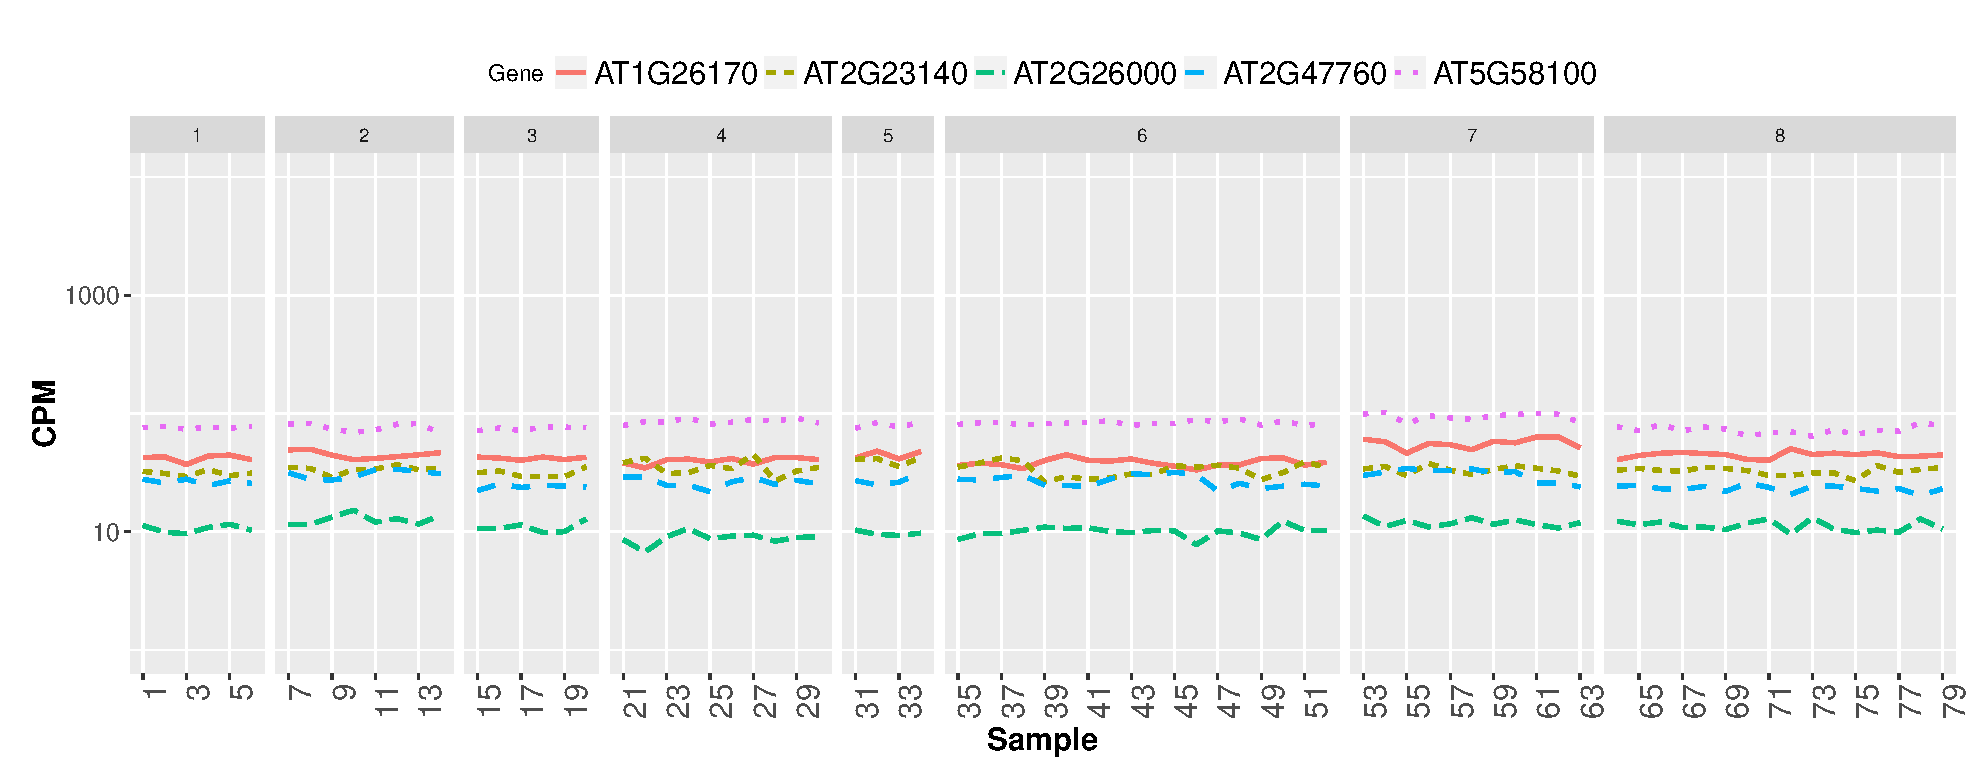
\includegraphics[width=15cm,height=6cm]{Figures/A3.eps}
	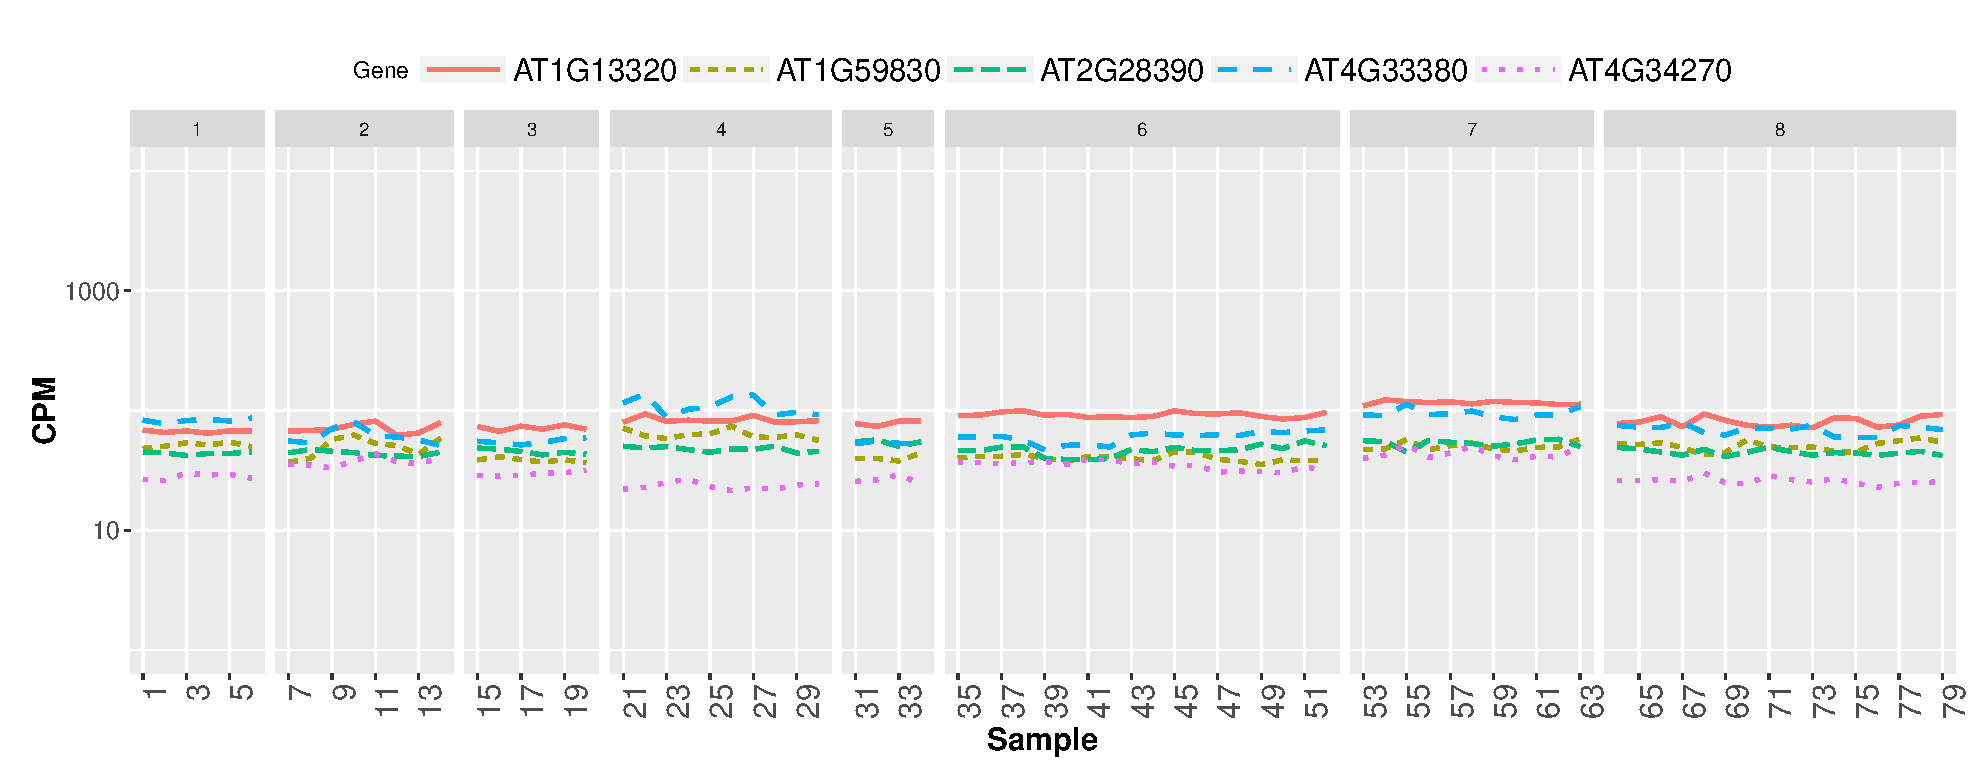
\includegraphics[width=15cm,height=6cm]{Figures/A2.eps}
	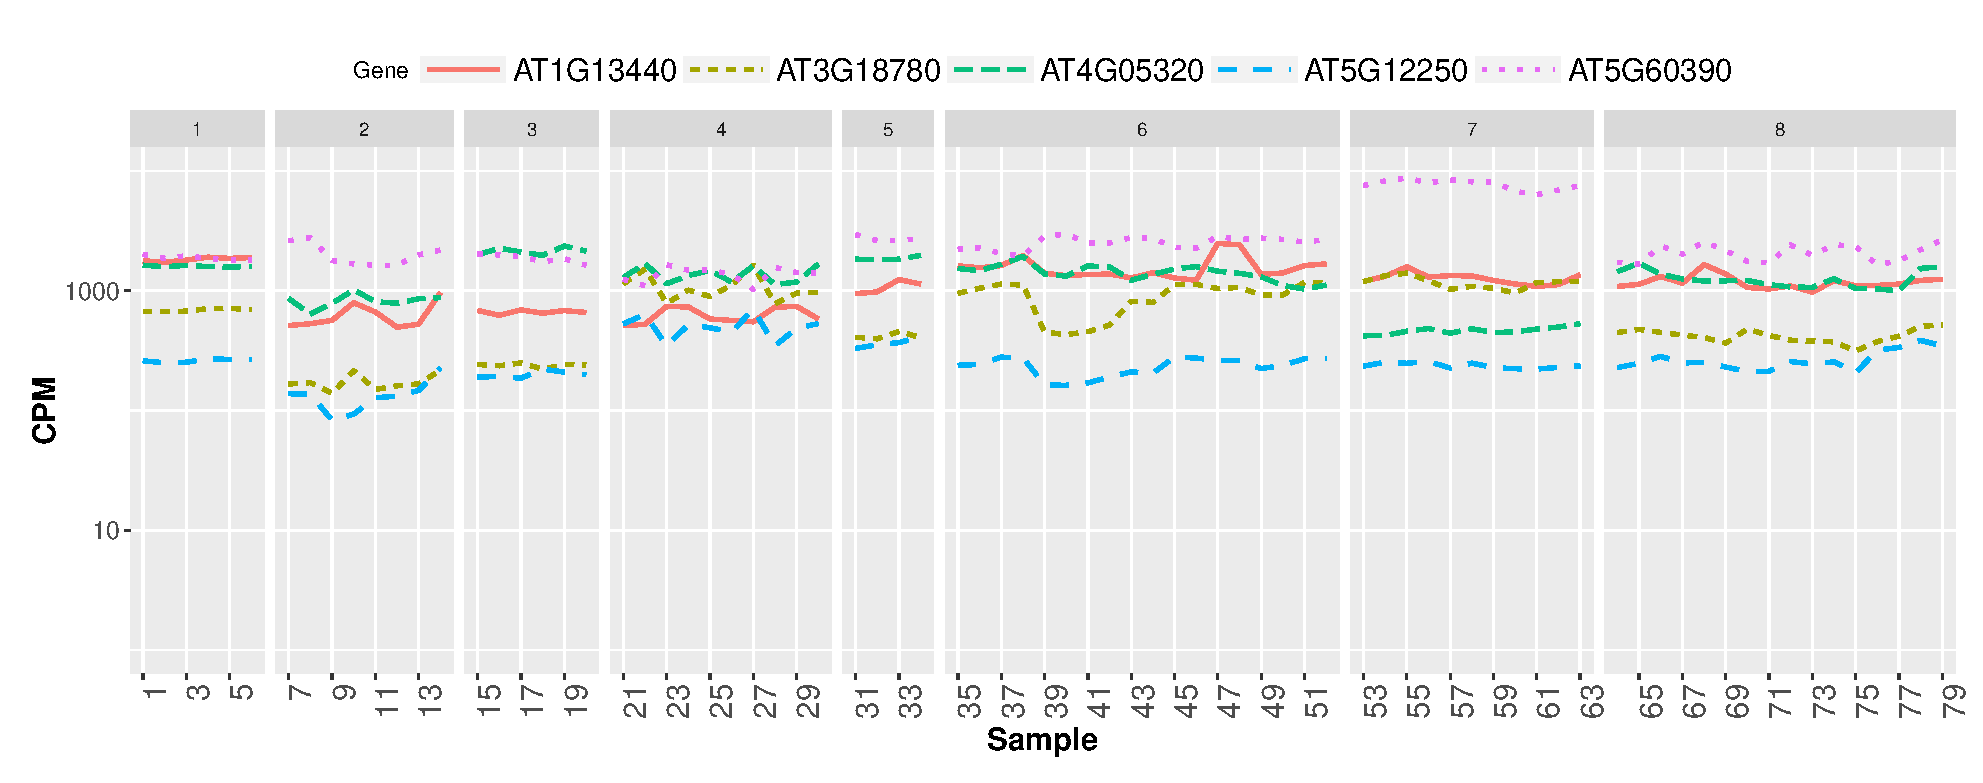
\includegraphics[width=15cm,height=6cm]{Figures/A1.eps}
	\caption{{\small{\label{expressinlevel1} Expression levels CPM of genes across RNA-Seq samples using multiple-tissue data: 5 stably expressed genes identified by our method(top)}; 5 stably expressed genes from developmental series by Czechowski et. al. (middle); 5 traditional reference genes (bottom).}}
\end{center}
\end{figure} 

% \subsection{Comparison of different stability measures}\label{section:stabilityMeasure}
\subsection{Factors affecting stability ranking}\label{section:stabilityMeasure}
The previous two subsections demonstrate that when using a numerical measure
to quantify gene expression stability, the outcome is dependent on 1) the
biological context reflected in the reference data sets used and 2) the
technology used for measuring gene expression. It should also be intuitive and
obvious, and we will further clarify in the second half of this subsection,
that 3) the stability ranking is also dependent on the specific numerical
measure used.  In this section, we will first compare the lists of
stably-expressed genes identified under different scenarios where one of more
of the above three factors differ.  We then further clarify the role of a
specific measure by comparing our stability measure, the total variance
$\sigma^2$ from the GLMM in equation \ref{eq:GLMM} of Section
\ref{subsection:OurMethod}, to geNorm $M$ value of
\cite{vandesompele2002accurate}. 

We look at an additional five lists of stably expressed genes identified under
different scenarios and examine how each of these five lists overlaps with the
the top stably-expressed genes identified from the multi-tissue group  of
RNA-Seq experiments  according to the total variance measure $\hat\sigma^2$
(see subsection 3.1 ??? \ref{section:DataCollection}). 
The five lists are: 
\begin{enumerate}
    \item[$L_1$:]
 100 top stably expressed genes from the multiple-tissue group according
 to the $M$ value in geNorm (applied to $\log(\text{count}+1)$); 
\item[$L_2$:]	
100 top stably expressed genes from the seedling group according to the total variance $\sigma^2$ from the GLMM;
\item[$L_3$:]
100 top stably expressed genes from the leaf group according to the total variance $\sigma^2$ from the GLMM; 
\item[$L_4$:]
100 stably expressed genes identified from a developmental series of microarray
experiments by \cite{czechowski2005genome} using the CV measure; 
\item[$L_5$:] 50 stably expressed genes identified by \cite{dekkers2012identification} from microarray
seed experiments using the CV measure.  
\end{enumerate}
In Figure \ref{fig:rankVSrank_RNA}, the plot the {\em recall} percentage for
each list above against the number of top stably-expressed genes we selected
as reference from the multi-tissue-type group. 
The recall percentage for $L_i$ is defined as 
\[ \frac{ \#	 \{L_i \cap \text{reference set} \}}{\# \{L_i\}}\times 100, \]
where $\#\{ \}$ denotes the number of elements in the list.
We have the following observations:
\begin{enumerate}
    \item
	The list $L_1$ is identified from the same set of RNA-Seq experiments as the
	reference sets, but using a different stability measure ($M$ value in
	geNorm). This list has significant overlap with the top
	stably-expressed genes identified using the total variance measure:
	$35$ and $97$ out of the $100$ genes from the list $L_1$ are among the
	top $100$ and $1000$, respectively, most stably-expressed genes from the
	multiple-tissue group identified using the total variance measure. 
    \item
	The lists $L_2$ and $L_3$ are identified from different sets of
	RNA-Seq experiments (leaf and seedling experiments) using the same
	stability measure as used for the reference sets. The lists $L_4$ and $L_5$ are
	identified from microarray experiments (a developmental series and a
	seed group) and using the CV measure. The overlapping (recall)
	percentages are still statistically significant, but much less than in
	the case of $L_1$.  This shows that differences in tissue type and in
	measuring technology both influence the expression stability rankings,
	and to comparable degrees. The lists $L_3$ and $L_5$ have the least
	overlapping percentages with the reference sets. Theses lists are
	identified from a leaf group and a seed group respectively.
	Our understanding is that the leaf group and the seed group are more
	biologically homogeneous than the multi-tissue group and thus provide
	very different biological contexts for evaluating expression stability.
\end{enumerate}

%(\textbf{use stably expressed genes from RNA-Seq study when studying RNA-Seqdata!, even if not the same tissue type}) Next, we compared the consistencybetween stably expressed genes identified from seedling, leaf and multiple-tissue in this study. Figure \ref{fig:rankVSrank_RNA} shows that stably expressed genes from RNA-Seq study are slightly more consistent than when comparing those from RNA-Seq data with those from microarray data, but less consistent than stably expressed genes identified from the same data with different stability measures.

%\textbf{Difference due to data sources}\\ Stably expressed genes may also vary due to different data sources. For those most stably expressed genes (top 100 in Czechowski et. al. and top 50 in Dekkers et. al., identified as stable from microarray data), only $< 40\%$ are present in top 1000 list from RNA-Seq data based on our stability measure (figure \ref{fig:rankVSrank_RNA}).

%\textbf{Difference due to biological functions}\\
% In pre-genomic era, HKGs are often believed to be stably expressed for biological reasons. HKGs are typically constitutive genes that maintain basic cellular function, and therefore are expected to express at relatively constant levels in non-pathological situations. However, stability in terms of biological functionality does not imply stability in terms of numerical expression values.  The data-driven methods are generally more reliable, as shown by various PCR validation experiments of microarray (\cite{czechowski2005genome} \cite{hruz2011refgenes}).

 \begin{figure}[h!]
 	\begin{center}
 		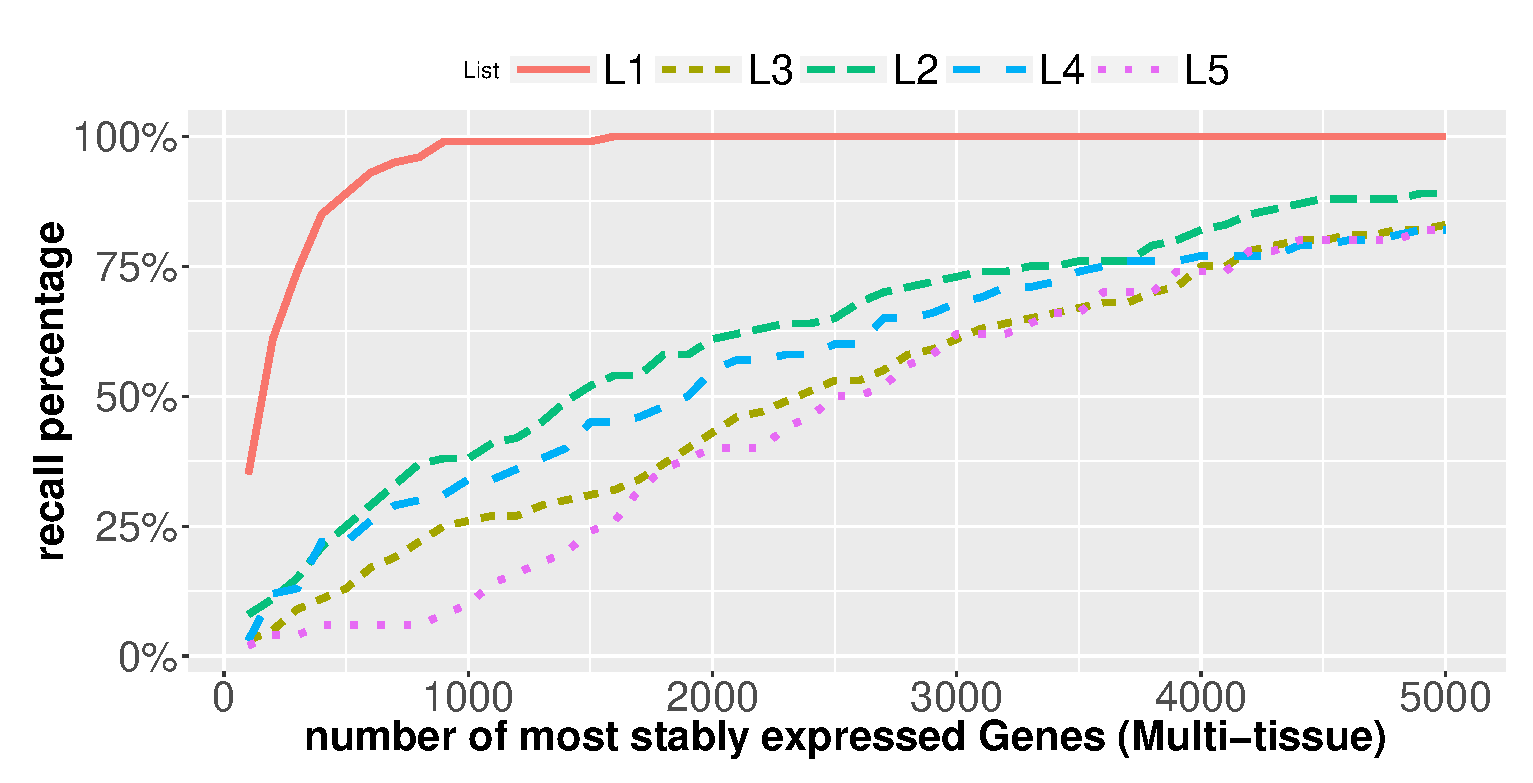
\includegraphics[scale=0.5]{Figures/rankVSrank_RNA2.eps}
 		\caption{percentage of occurance. For each of case C1)--C5), we choose top 100 stably expresed genes, except Dekkers(2012) where only a list of 50 genes is available. $x$-axis is the number of most stably expressed genes and $y$-axis shows the percentage of occurance.}
	 	\label{fig:rankVSrank_RNA}
	 	\end{center}
 \end{figure}
When applied to the same set of experiments, the $M$ value and total variance
measure $\hat\sigma^2$ give similar expression stability rankings. 
This comes as no surprise because M-value and
normalization step needed for computing our total variance measure have the
same fundamental assumption. The basic principle
behind the $M$-value is that the expression ratio of two stably-expressed
genes should be identical in all samples. In formula, it means that the
expression values of two genes $i_1$, $_2$ in any two samples $j_1$, $j_2$
should satisfy
\begin{equation}\label{eq:typical}
   \dfrac{y_{i_1, j_1}}{y_{i_2, j_1}} = \dfrac{y_{i_1, j_2}}{y_{i_2, j_2}}.
\end{equation} 
(In practice, genes  with the more ``typical'' expression profiles are
considered as more stable.)
Our total variance measure $\hat\sigma^2$ is estimated from normalized data.
The basic assumption in the normalization method is that majority of genes are
not DE. In formula, it means for any stably-expressed gene $i_1$, its expression
level as measured by the relative frequency should be stable across all
samples,
\begin{equation}\label{eq:DESeq} 
    \frac{y_{i_1j_1}}{S_{j_1}}= \dfrac{y_{i_1j_2}}{S_{j_2}},
\end{equation}
where $S_{j_1}$ to $S_{j_2}$ are the normalized library sizes (i.e., $R_j N_j$ in equation).
This implies for any two stably-expressed genes $i_1$ and $i_2$
\begin{equation}\label{eq:DESeq2} 
    \frac{y_{i_1j_1}}{y_{i_1j_2}} = \frac{y_{i_2j_1}}{y_{i_2j_2}} =
    \frac{S_{j_1}}{S_{j_2}}.
\end{equation}
This first equation in \ref{eq:DESeq} is equivalent to equation
\ref{eq:typical}.

[The iterative elimination procedure]
Note that in the geNorm program by \ref{ }, an iterative elimination procedure
is applied to a given reference set to determine final ranks of the expression
stability. We did not use such an iterative procedure in the comparisons
above.  

This iterative procedure creates an extra layer of complexity.  We note that
the iterative elimination procedure can give surprising results and the
adaption of it in practice should not be automatic.  We demonstrate the
effect/behavior of iterative elimination procedure by a toy example in Table
\ref{table:toyexample} below, where an artificial data set is created with two
samples, each containing seven genes. Columns 2 and 3 are the expression
values, column 4 is the gene ranking according to the $M$ value (geNorm
without iterative elimination), and column 5 is the ranking by the geNorm
(with iterative elimination). In this example, the initial rankings according
to the $M$-value is very difficult from the final rankings after the iterative
elimination. Once a less stable gene is eliminated, the rankings of the rest
genes can change dramatically. This behavior makes it difficult to predict the
final rankings. \dots

  
The $M$ value and the geNorm differ in ranking Gene1 --- Gene5, where Gene4
and Gene5 are ranked first by the $M$ value and Gene1 and Gene2 are ranked
first by the geNorm. For the geNorm, while Gene4 and Gene5 are ranked first in
the begining, their rankings immediately drop to 4 and 5 after Gene7 is
eliminated. At each iteration, the geNorm removes one gene that deviates the
most from the others. As the iteration continues, the remaining genes become
more similar to each other. The end result is that genes with the most typical
expression pattern are ranked in the top (Gene1 --- Gene3 in this example). 	  

Effectively, the iterative procedure is using a different reference set (with
decreasing size) in each iteration.

\begin{table}[ht]
	\centering
	\begin{tabular}{rrrrr}
		\hline
		 & \multicolumn{2}{c}{Raw Counts} & \multicolumn{2}{c}{Rank}\\
	Gene	& sample 1 & sample 2 & $M$ value & geNorm \\ 
		\hline
		Gene1 & 1 & 1 & 3 & 1 \\ 
		Gene2 & 1 & 1 & 3 & 1 \\ 
		Gene3 & 1 & 1 & 3 & 3 \\ 
		Gene4 & 1 & 2 & 1 & 4 \\ 
		Gene5 & 1 & 2 & 1 & 5 \\ 
		Gene6 & 1 & 3 & 6 & 6 \\ 
		Gene7 & 1 & 4 & 7 & 7 \\ \hline 
	Library Size & 7 & 14 & & 	\\
		\hline
		\end{tabular}
		\caption{Toy Example} 
		\label{table:toyexample}
		\end{table}

\begin{table}[ht]
	\centering
	\caption{Toy example}
	\label{table:toyexample2}
	\begin{tabular}{rrrrrrrr}
		\hline
	Gene & \multicolumn{2}{c}{Raw Counts} & \multicolumn{2}{c}{Relative Frequency (DESeq)} & \multicolumn{3}{c}{Rank} \\
		& sample1 & sample2 & sample1 &sample2 & GLMM & Vvalue (geNorm) & geNorm \\ 
		\hline
		Gene1 & 1 & 1 & 0.143 & 0.071 & 3 & 3 & 1 \\ 
		Gene2 & 1 & 1 & 0.143 & 0.071 & 3 & 3 & 1 \\ 
		Gene3 & 1 & 1 & 0.143 & 0.071 & 3 & 3 & 3 \\ 
		Gene4 & 1 & 2 & 0.143 & 0.143 & 1 & 1 & 4 \\ 
		Gene5 & 1 & 2 & 0.143 & 0.143 & 1 & 1 & 5 \\ 
		Gene6 & 1 & 3 & 0.143 & 0.214 & 3 & 6 & 6 \\ 
		Gene7 & 1 & 4 & 0.143 & 0.286 & 7 & 7 & 7 \\ 
		\hline
	\end{tabular}
\end{table}




%With the same RNA-Seq data, we identified top 1000 stably expressed genes for both geNorm and NormFinder algorithms. There is substantial consistency (Figure \ref{fig:wenn}) between different stability measures. For example, the agreement between geNorm and our method suggests that the most typical expression pattern is stable expression (i.e., has low variance in the estimated log relative mean of normalized counts). 

%\begin{figure}
%\centering
%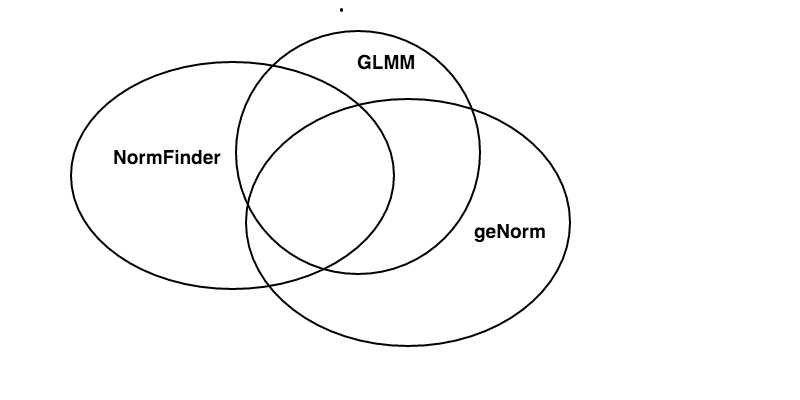
\includegraphics[width=0.7\linewidth]{Figures/wenn.eps}
%\caption{Overlap diagram: each circle represents top 1000 stably expressed genes from geNorm, NormFinder and our method}
%\label{fig:wenn}
%\end{figure}


\subsection{Sources of variation}\label{Section:varianceComp}
% One nice feature about random effects model (\ref{eq:GLMM}) is that it allows us to
% decompose total variance into 3 variance components for each gene. With the
% variance components estimated, we are able to tell how much each component
% contributes to total variation.  

For each gene, the GLMM (equation \ref{eq:GLMM}	of section \ref{subsection:OurMethod}) allows us to decompose
total count variance into between-sample, between-treatment and
between-experiment variance components. The estimated variance components tell us how much each component contributes
to the total variation. Table \ref{table:percentageofvariation} summarizes the percentages of the total variation attributable to each of the three components averaged over all genes. Figure \ref{fig:densityplot} shows the histograms of the percentages. We also randomly select 20 genes from the top 1000 stably expressed ones, and 20 from all the genes of the multiple-tissue group. Figure \ref{fig:all} shows the stacked bar plot of variance components for each of the 40 genes.
As expected, the between-experiment variance component, on average,
explains the largest proportion of the total variation. In the group of leaf
experiments, the between-treatment variation is markedly greater than the
between-sample variation: one implication is that DE is easier to detect in
this group of experiments.  [Ask Jeff] Our intuition is
that leaf samples tend to be more homogeneous and thus the treatment effect is
easier to detect between leaf samples. (The larger component of
between-treatment variation suggests the existence of a higher proportion of
DE genes.) 
 
 \begin{center}
 \begin{table}[h!]
 	\centering
 	\caption{proportion of estimated variance components}
	 \label{table:percentageofvariation}
 	\begin{tabular}{lrrr}\hline
 		& Seedling & Leaves & Multiple-tissue \\  \hline
 		between-sample     & 12.3\%   & 16.0\% & 8.4\%           \\
 		between-treatment  & 13.4\%   & 28.0\% & 6.6\%           \\
 		between-experiment & 74.3\%   & 56.0\% & 85.0\%         \\ \hline
 	\end{tabular}
 \end{table}
\end{center}

 \begin{figure}[h]
\begin{center}
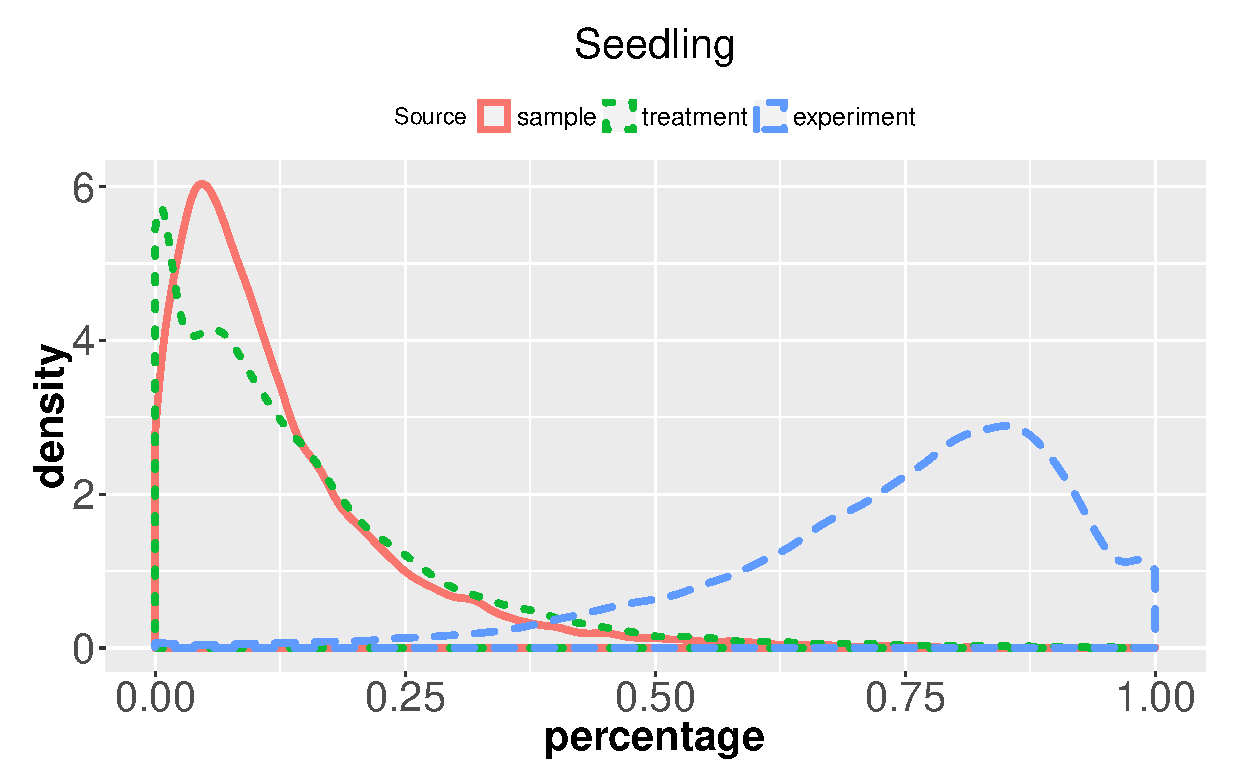
\includegraphics[width=5cm,height=4cm]{FiguresTest/var_dens1.eps}
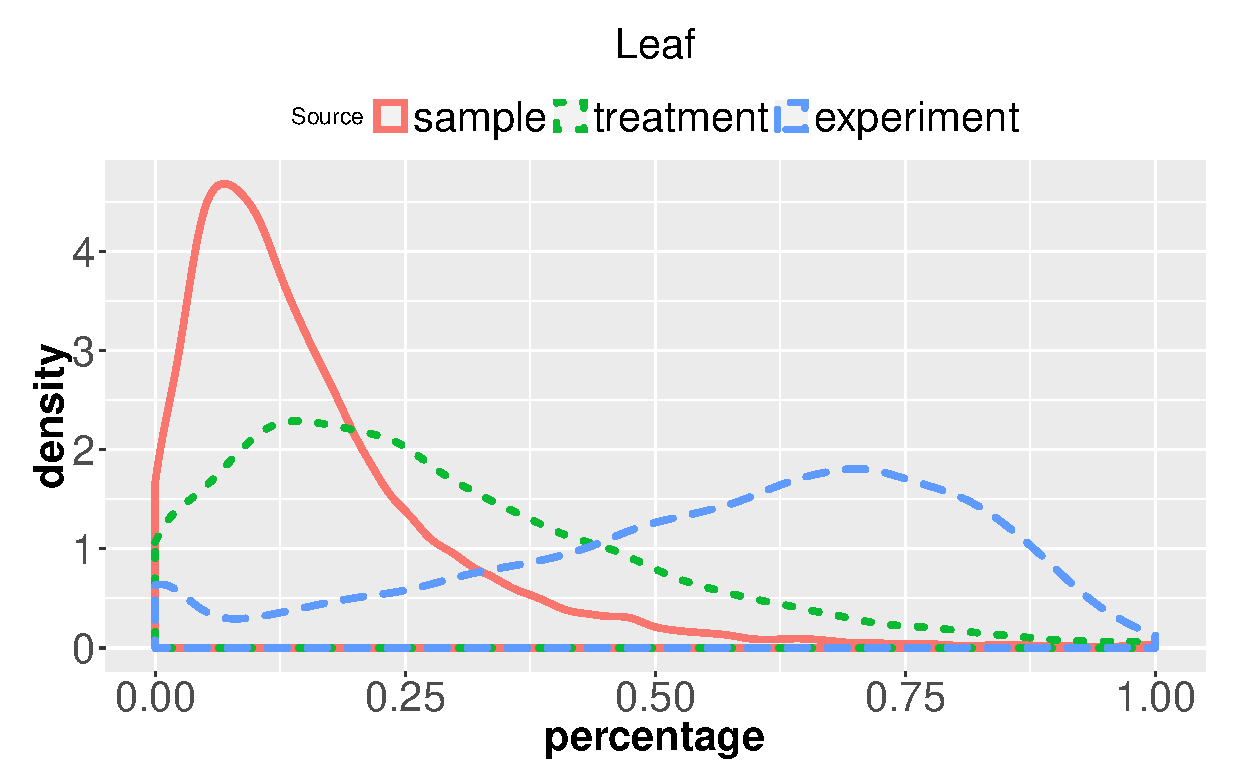
\includegraphics[width=5cm,height=4cm]{Figures/var_dens2.eps}
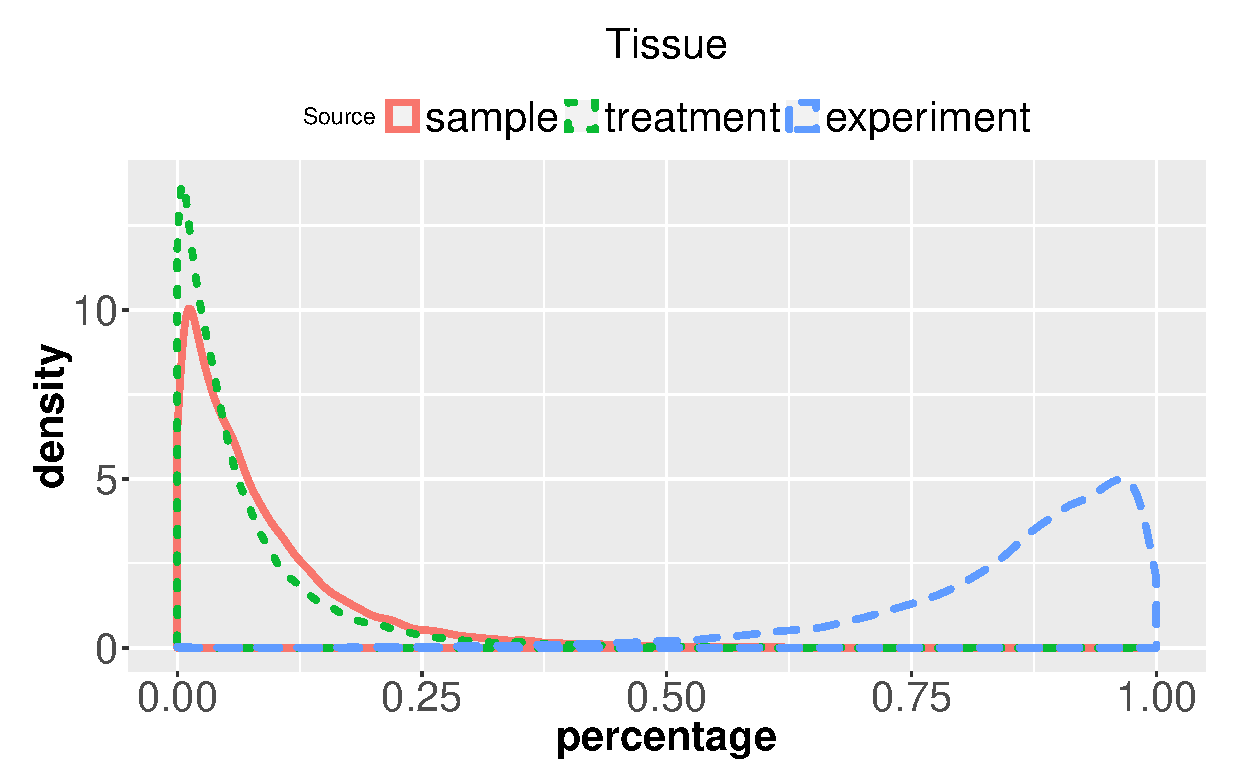
\includegraphics[width=5cm,height=4cm]{Figures/var_dens3.eps}
\caption{ Density plot of variance component: Seedling data, Leaf data, Tissue data (left to right).}
\label{fig:densityplot}
\end{center}
\end{figure} 


\begin{figure}[!h]
	\centering
	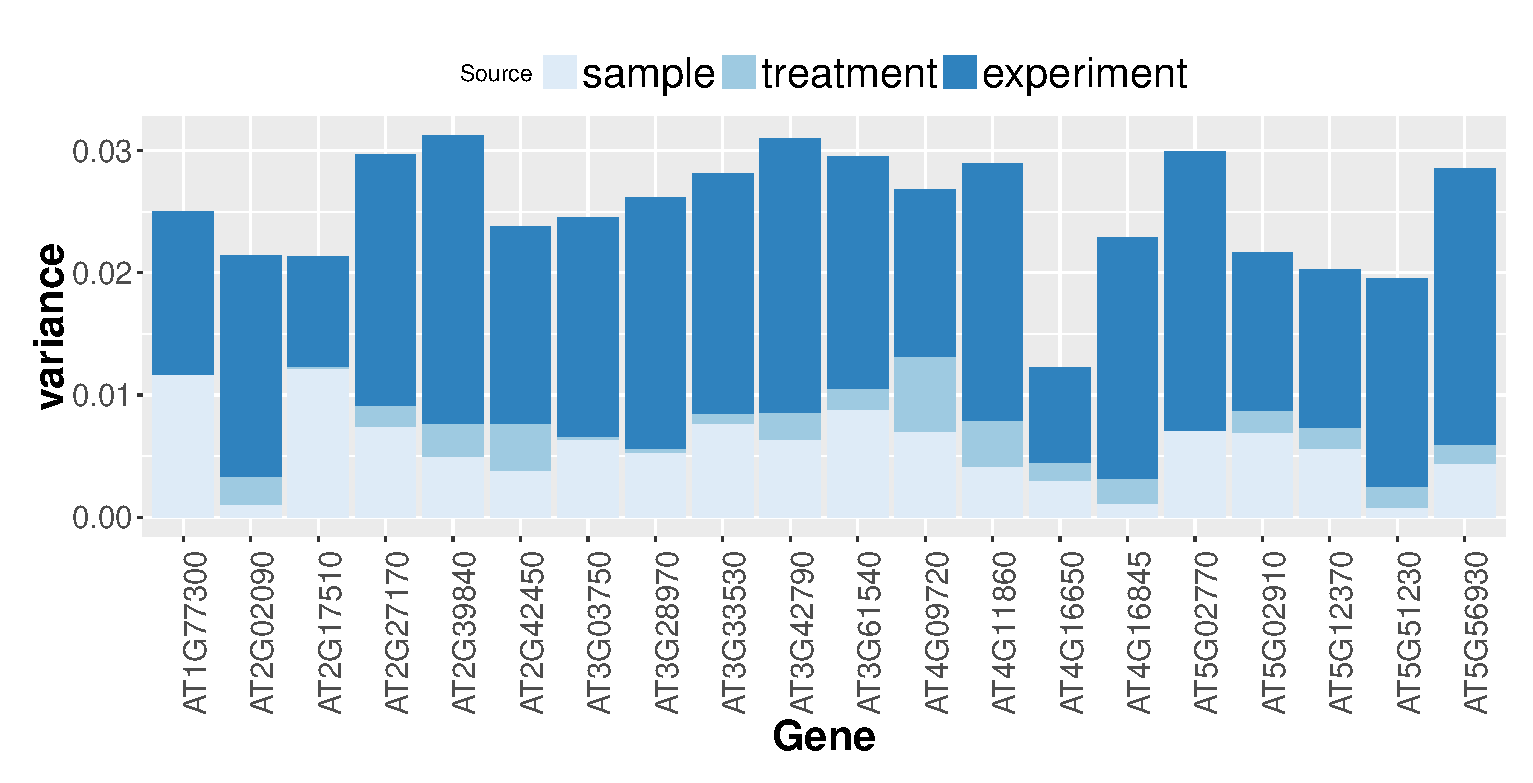
\includegraphics[width=0.8\linewidth]{Figures/top1000.eps}
	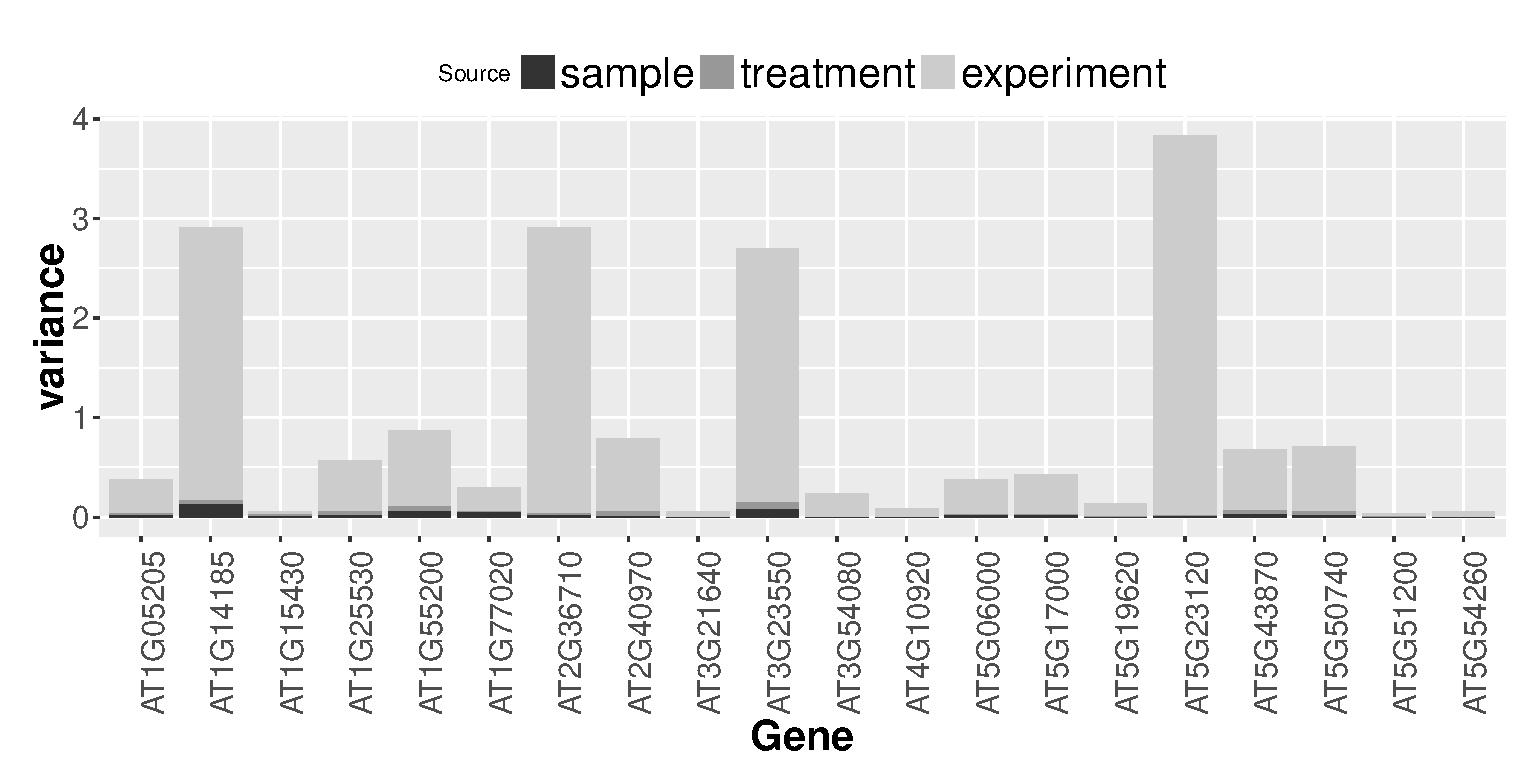
\includegraphics[width=0.8\linewidth]{Figures/all.eps}
	\caption{stacked bar plot of variance components. Left: 20 stably expressed genes randomly selected from top 1000; right: 20 genes randomly selected from all the genes.}
	\label{fig:all}
\end{figure}




\subsection{A common reference set of genes for normalization}\label{Section:commonReference}
One goal of identifying stably expressed genes is to use them as reference genes for normalization. We used stably expressed genes to see how normalization factors vary by choosing different sizes of reference set.   As an illustration, we chose top 10, 100, 1000, 10000 stably expressed genes as reference, and then calculated normalization factors by DESeq method for each sample in seedling, leaf and multiple-tissue group, respectively. Figure \ref{fig:normfactor} shows paired scatter plot of normalization factors, in which high consistency is reached when top 100 or 1000 stably expressed gene are selected. We thus recommend using top 1000 stably expressed genes as reference to compute normalization factors. %A common reference set of stably expressed genes will help improve comparability of the data sets and interpretability of DE test leaf.



 \begin{figure}[h!]
\begin{center}
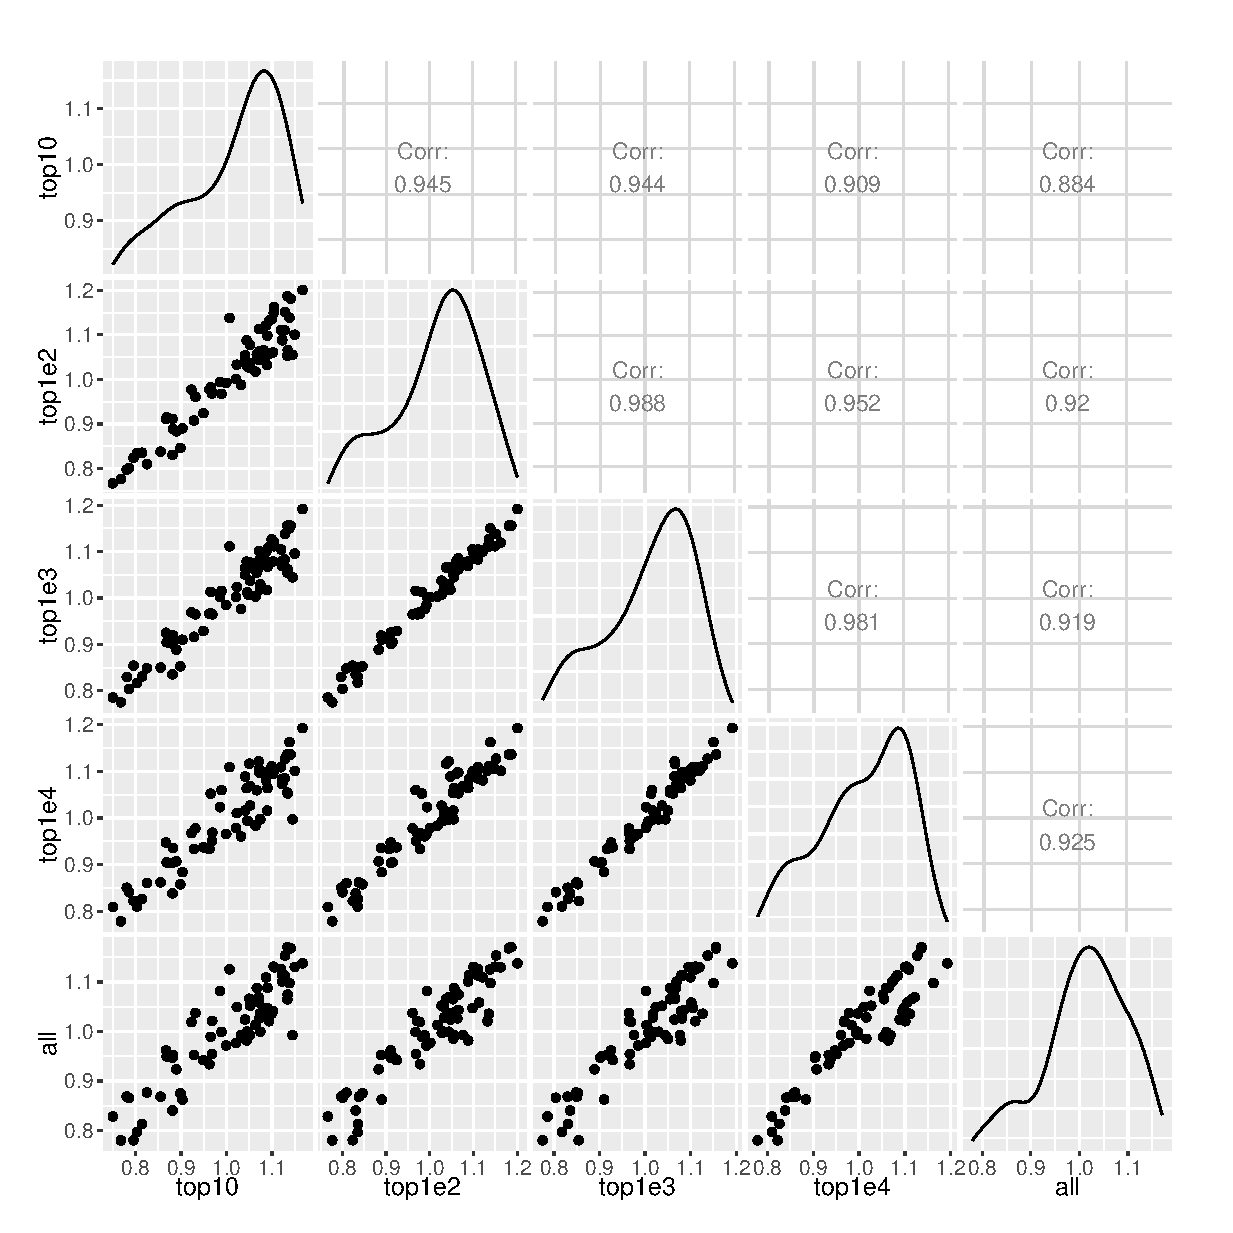
\includegraphics[scale=0.2]{Figures/norm1.eps}
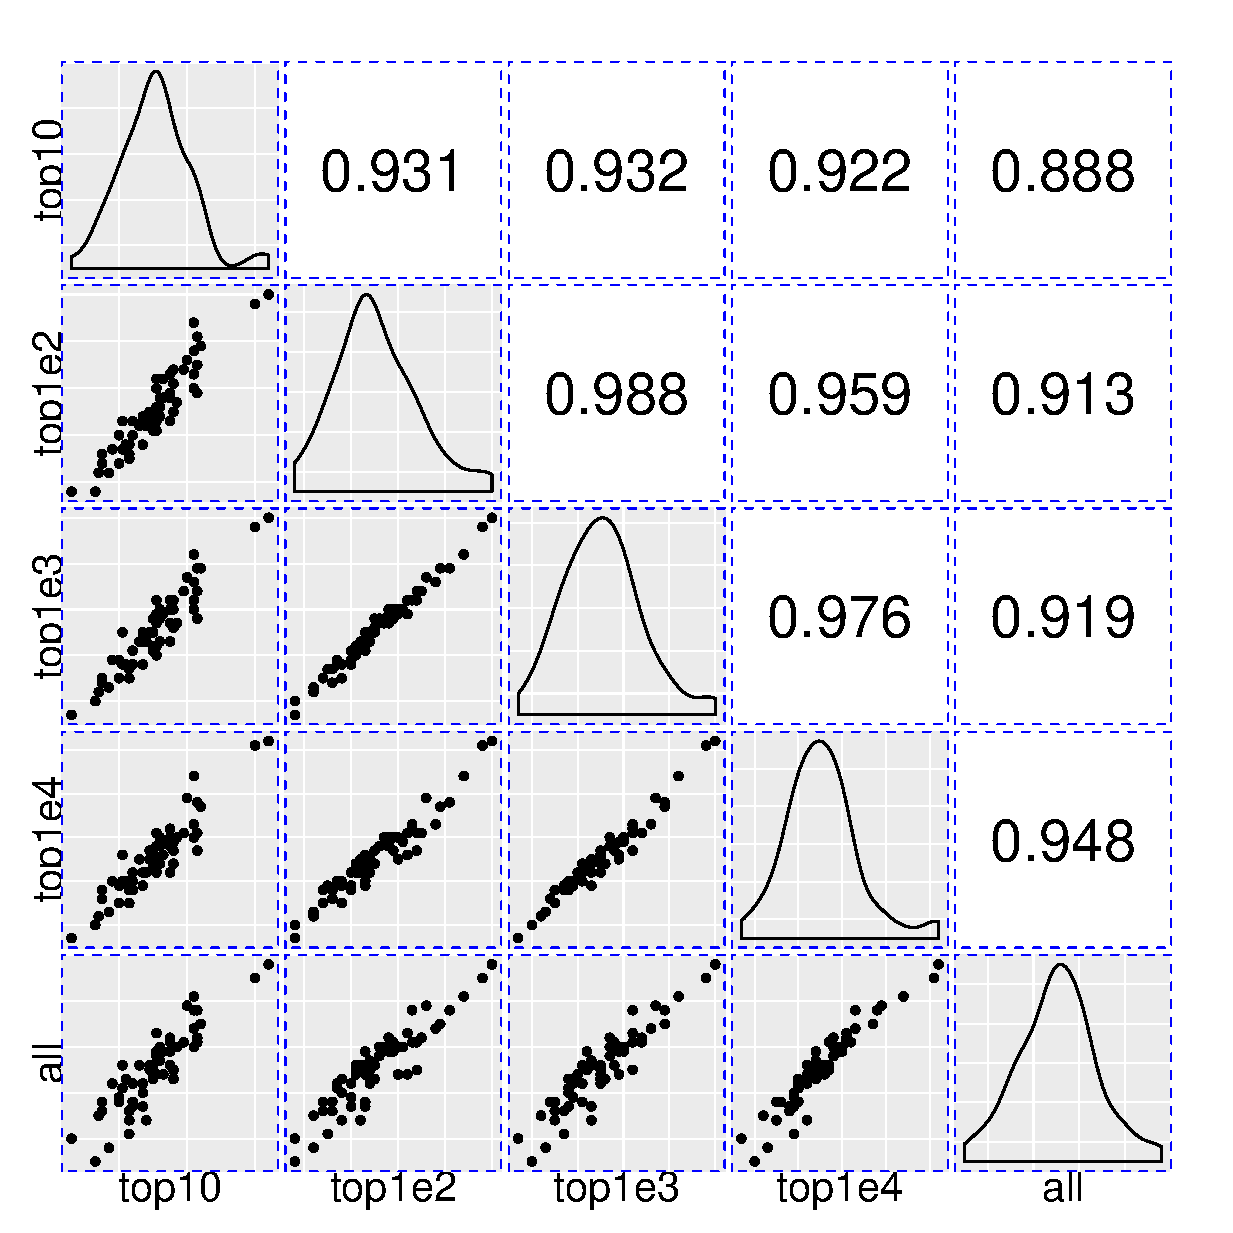
\includegraphics[scale=0.2]{Figures/norm2.eps}
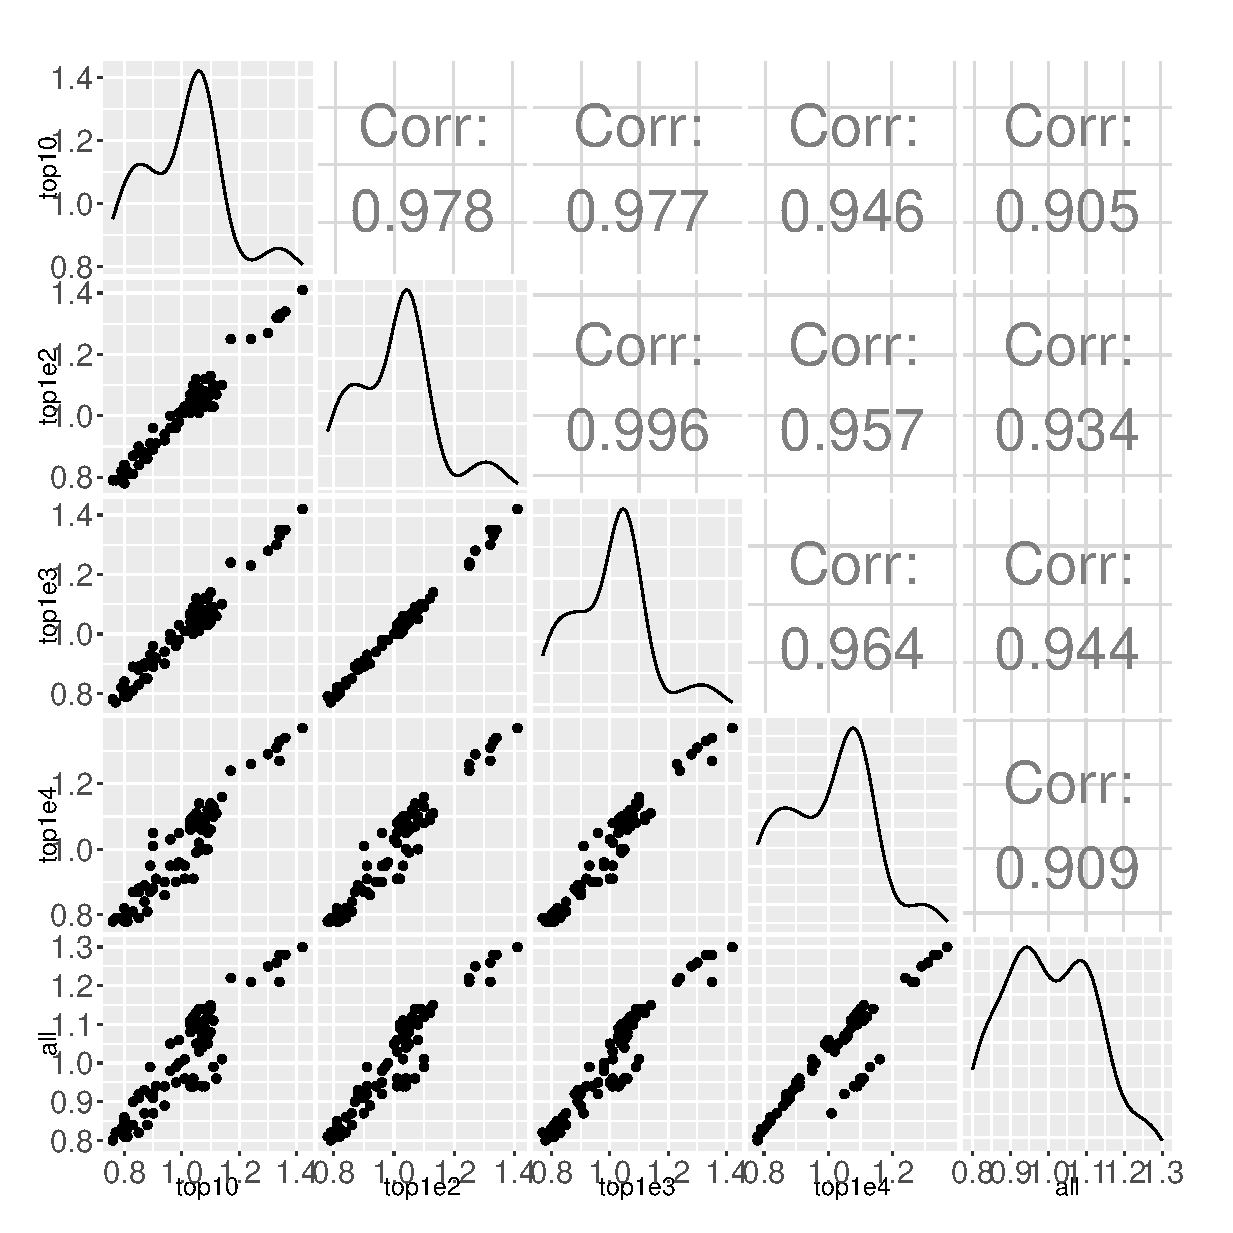
\includegraphics[scale=0.2]{Figures/norm3.eps}
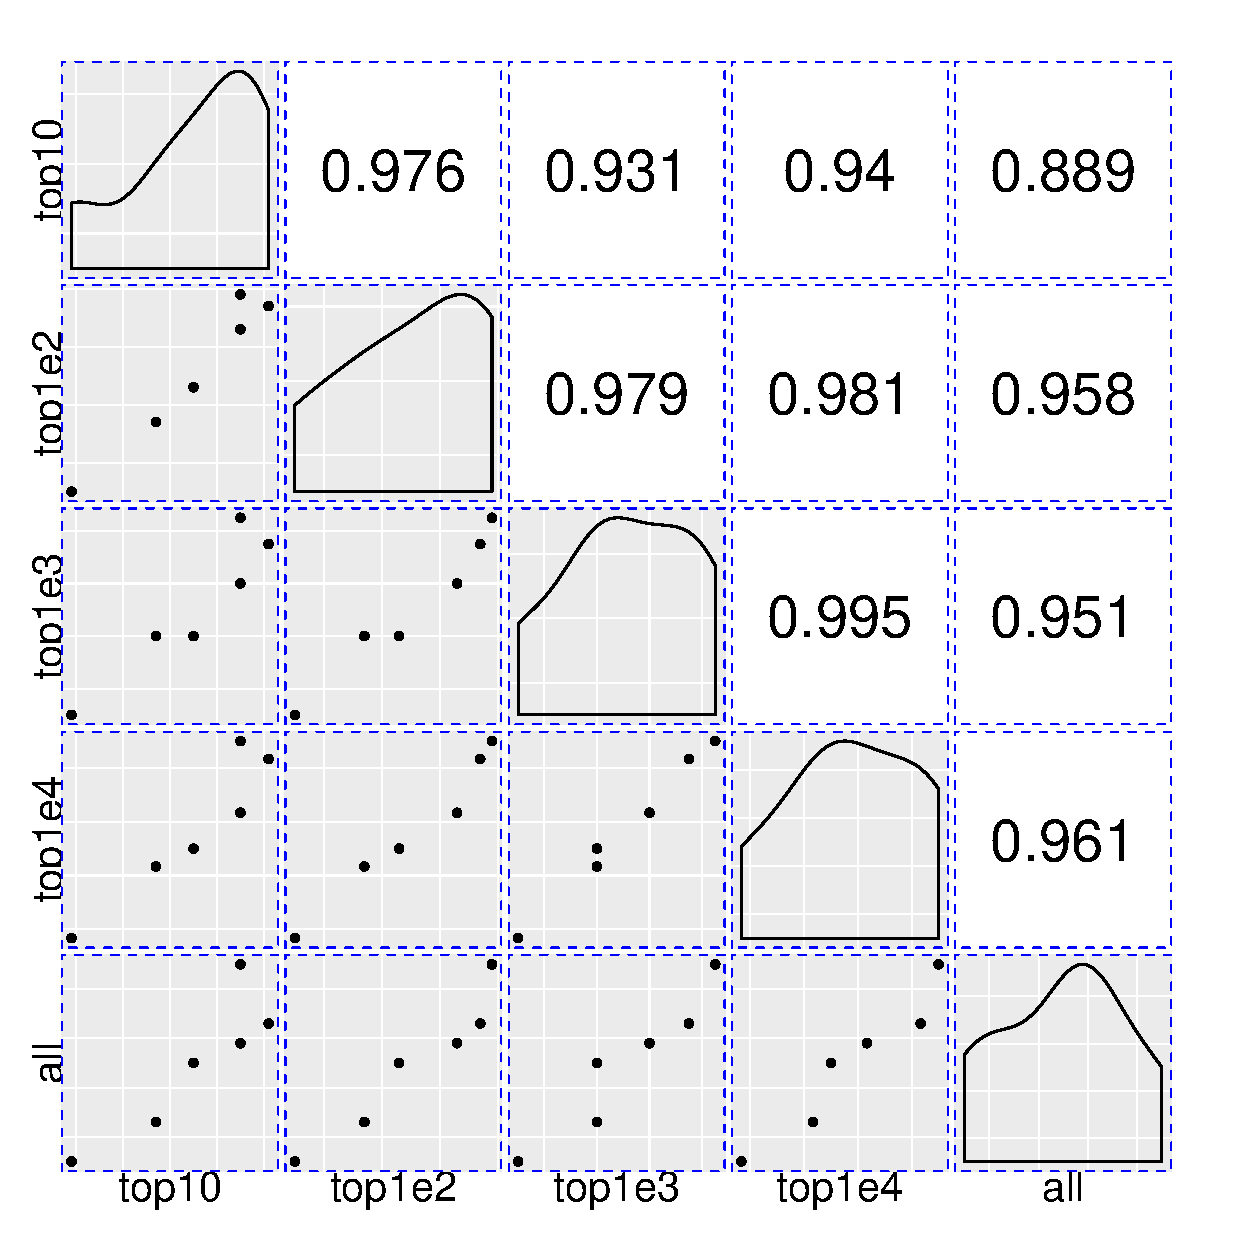
\includegraphics[scale=0.2]{Figures/norm4.eps}
\caption{\label{fig:normfactor} matrix plot of normalization factors by choosing top 10--10000 stably expressed genes for seedling group (top left), leaf group (top right), multiple-tissue (bottom left) group. The bottom right plot shows the normalization factors of a new seedling experiment GSE66666 (sample size is 6) when using top 10--10000 stably expressed genes from seedling group.}
\end{center}
\end{figure}

  \section{Discussion}
In this paper, we advocate quantifying gene expression stability by applying a
numerical stability measure to a large number of existing data sets.  This
strategy has also been used by many for finding stably expressed genes using
microarray data.  When using such a strategy, the outcome is determined by two
factors: the data sources used and the specific numerical stability measure.
We emphasize that numerical stability is not equivalent to biological
stability (??? Jeff).  (Ask Jeff about  ``biological stability'': do
biologists talk about ``biological stability''?) For example, we demonstrated
that the expression levels of traditional house-keeping genes are not
necessarily stable according to a numerical measure. 
Biological stability is a vague term and not easy to quantify.  Numerical
stability is generally more tractable. (Some have argued that numerically
identified stably expressed genes are more reliable. We feel that argument is
somewhat circular??? The same numerical measure is used to both identify the
stably expressed genes and to verify their stability.) It should be obvious
but worth emphasizing that 1) different stability measures will give rise
different ranking of gene stability and 2) the stability measure will also
depend on the technology used for measuring gene expression: for example,
microarray data and RNA-Seq data will give different sets of stably expressed
genes.


  \textbf{Major findings of the study}
  Normalization is an essential step for accurate inference in RNA-Seq data analysis. Global normalization methods may lead to erroneous conclusions when they rely on inappropriate reference genes. In this study we identified three sets of stably expressed genes for different organs and tissues of Arabidopsis. We conclued that traditional HKGs are not necessarily stable under not only microarray, but also in RNA-Seq experiment when they are evaluated by numerical stability measures. While \cite{czechowski2005genome} identified novel reference genes for different experimental conditions, we demonstrated that they are not among the best candidates for RNA-Seq study. We recommend a set of 1000 reference genes to calculate normalization factors for RNA-Seq data.  
   
%   We find that variation in Arabidopsis RNA-Seq experiment is dominated by lab effects. In this paper, random effects model allows us to quantify  between-lab, between-treatment and between-sample variance components for each gene.On average, between-lab variance can account for 52.8\% to 76.7\% of total variation. The second important source of variation comes from treatment effect (16.2\% - 25.0\%) and biological sample variation is the smallest. 



\subsection{Moved from Introduction part}



(To Discussion ???) {\bf Further discussion} Previous studies showed that
normalization are needed to account for nuisance effects, including
\textit{between-sample} effects, e.g., sequencing depths, flow-cell/library
preparation effects (\cite{bullard2010evaluation},
\cite{robinson2010scaling}), as well as \textit{gene-specific} effects, e.g.,
gene length or GC-contents (\cite{risso2011gc}, \cite{hansen2012removing}). A
number of normalization approaches are proposed to address different types of
unwanted nuisance effects (\cite{dillies2013comprehensive},
\cite{risso2014nat}). Different from global-scaling normalization,
\cite{risso2014nat}  proposed a regression-based normalization-remove unwanted
variation (RUV).  In that paper, they regressed the read counts on the known
covariates of interest (e.g. treatment effects) and unknown factors of
nuisance effects. The factors of nuisance effects are estimated from a subset
of data, and are then adjusted for in DE analysis. In RUVg approach, they are
estimated through a factor analysis. A main assumption for RUVg is that a set
of stably expressed genes can be identified first.


\textbf{Why is stably expressed gene important/difficult} Count normalization would have been easy if one could identify and use as reference a set of stably expressed genes whose expression levels are known or expected to not vary much under different experimental conditions.  Effectively, TMM or DESeq method use genes with relatively small observed fold changes under a single experiment as a reference gene set in normalization. There are two obvious issues with this strategy: 1. The available sample size in any single experiment may be too small for us to reliably estimate true fold changes. 2. If the experiment condition can affect expression levels of more than half of the genes (\cite{loven2012revisiting}, \cite{wu2013use}), many of the existing normalization methods (???) may be unreliable.  


To identify a set of stably expressed genes, our method still need to estimate an initial set of normalization factors where we need to make assumptions about relative fold changes between samples. This kind of circular dependence seems unavoidable \citep{vandesompele2002accurate}. Our stretagy is to use an iterative procedure: we rank all the genes based on our stability measure, and use top 1000 stably expressed genes to calculate normalization factors, which are the new offsets in the next iterative GLMM estimating procedure. After five iterations, the top 1000 genes have a large overlap (90.9\%) with the top 1000 genes from the first iteration. In practice, we recommend one iteration to be enough.  


Stably expressed genes may or may not be the most stably expressed ones for a
particular experiment when they are identified by pooling multiple
experiments. (Discussion) Two subtle points we want to make: 1) using an explicit reference set improves interpretability of DE test leaf; 2) using a common reference
set improve comparability when analyzing two or more data sets. (moot ???)
\dots Another subtle point we want to make is that a reference set does not
have to be absolutely stable to be useful as a reference set: we can slightly
change our perspective and interpret all DE leaf as relative to the
reference set.  ??? For example, a fold change of 2 can be interpreted as the
fold change of this gene is 2 more than those genes in the reference set. ???
Any of the simple normalization methods discussed earlier (REFs) are
effectively specifying an implicit set of genes as a referent set. Our
proposal is to make the reference set explicit to improve interpretability of
the leaf.  Furthermore, using an explicit common reference set becomes more
useful when the interest is in comparing different experiments. For example,
when two RNA-Seq data sets are separately normalized with different reference
sets, a fold change of two observed in one experiment may not be directly
comparable to a fold change of two observed in the other.  This concern can be
alleviated by using a common set of reference genes.
Different estimated normalization factors effectively specify a different
reference set \ldots (Improve intepretability and comaprability)



% Using a common reference set for count normalization can improve comparability and interpretability.  


% RNA-Seq is superior to microarray technology because
% of its high-throughput, pricise measurement, as well as sensitivity for gene
% expressed at both low and very high levels \citep{wang2009rna}. 


% Typically, large sets of microarray data are compiled for a given experimental
% condition, and stably expressed genes are validated and recommended for
% potential use. 


(???) Furthermore, new biological insights (REFs) \dots Stably expressed genes
are likely to be involved in basal metabolic or ‘house-keeping’ functions, such
as  kinase activity, nucleotide binding and protein modification processes.
\cite{sekhon2011genome} and \cite{wang2010dynamic} showed that stably
expressed genes are involved in biological processes included cellular
processes, transport, protein modification, translation and signal
transduction by Gene Ontology enrichment analysis. Besides, in expression
study, a high correlation between translational signiture and mRNA level is
found in human stably expressed genes\citep{line2013translational}. In that
paper, a significant increase in mRNA variation prediction was obtained by
selecting genes that are stably expressed in more than 1 tissue.\\




  \subsection{Alternative method}
Another widely adopted approach of fitting GLMM to the data is via negative binomial (NB) regression. In many cases,  RNA-Seq data analysis begins with the assumption that $Y_{jkl}$ follows a negative binomial distribution (a.k.a Poisson-Gamma mixture). The NB model introduces a dispersion parameter to capture the extra-Poisson biological variation.  In NB regression, we estimate between experiment and between treatment variation. Specifically,  for each gene, we assume $Y_{jkl}\sim NB(\mu_{jkl}, \phi)$ with the link function
 \[\log(\mu_{jkl})= \xi + \log(R_{jkl}N_{jkl}) + \alpha_l + \beta_{k(l)}\]
where similarly, $\alpha_l$ is the random effect for experiment, and $\beta_{k(l)}$ is random treatment effect nested in experiments.  The only difference is that the dispersion $\phi$, rather than variance of biological sample in Poisson regression, is estimated in NB setting. We saw no significant difference in estimating the variance components between these two approaches. The NB regression is run by \verb"glmer.nb()" in \verb"lme4" package\citep{bates2012lme4} and \verb"glmmadmb()" in \verb"glmmADMB" package\citep{bolker2012getting}. Unfortunately, both implementations of NB regression experienced convergence failure when modeling over 20,000 genes. \\

A limitation of this study is that the inherent design structures are not taken into account unless when the experiment is a case-control (single factor) study. Our concern is two fold: one, although we collected more than 150 samples, they are far from enough for a complicated design structure because usually there are only 2 or 3 replicates within each treatment;  two, efficient algorithm is not available for generalized linear mixed model with more than three random effects \citep{bolker2009generalized}. However, model (\ref{eq:GLMM}) is sufficient for the purpose of identifying stably expressed genes in this paper.



\section{Appendix}


\subsection*{ Estimation of Variance Components and Identification of Stably Expressed Genes}



The estimation procedure starts from the joint density function of $\bm Y=(Y_{jkl})'$ given $\bm \mu= (\mu_{jkl})'$, 
\[f(\bm Y|\bm \mu )=\prod_{ j, k,l}f(y_{jkl}|\mu_{jkl})=\prod_{j,k,l}\frac{[\mu_{jkl}]^{y_{jkl}}\exp(-\mu_{jkl})}{y_{jkl}!}\]
A re-expression of  (\ref{eq:GLMM}) in matrix form gives 
\[\log\bm \mu= \bm \xi + \log{\bm{NR}} + \bm {Z_1\alpha} + \bm{Z_2\beta} + \bm \epsilon \]
where $\bm \xi = \bm 1\cdot\xi$ and $\bm 1$ is a vector of 1s, $\bm Z_1$ is the design matrix for random effects $\bm \alpha=(\alpha_l)$, and $\bm Z_2$ is the design matrix for random effects $\bm \beta $. 
Therefore  $\bm\mu  \sim \log N(\bm \mu_0, \bm \Sigma)$ where 
$$\bm \mu_0 =\bm\xi + \log(\bm {NR}),$$ 
$$\bm \Sigma = \sigma_1^2\bm {Z_1Z_1'} + \sigma_2^2\bm {Z_2 Z_2'} +\sigma_0^2 \bm I$$
and $\bm I$ is an identity matrix of dimension $Q$ where $Q$ is the total number of biological samples. 
And 
\[f(\bm \mu |\bm \mu_0, \bm \Sigma)=\prod_{j,k,l} \mu_{jkl}^{-1}\cdot \frac{1}{ \sqrt{(2\pi)^Q|\bm\Sigma|}}\exp[-\frac{1}{2} {(\log\bm \mu - \bm \mu_0)^T\bm \Sigma^{-1}(\log\bm \mu - \bm \mu_0)}]\]
the joint density is then
\[f(\bm Y, \bm \mu |\bm \mu_0, \bm \Sigma) =\frac{1}{\sqrt{(2\pi)^Q|\bm \Sigma|}}\exp[-\bm 1^T\bm \mu - -\frac{1}{2} {(\log\bm \mu - \bm \mu_0)^T\bm \Sigma^{-1}(\log\bm \mu - \bm \mu_0)}]\prod_{jkl}\frac{[\mu_{jkl}]^{y_{jkl}-1}}{y_{jkl}!}\]
Therefore the likelihood function or the marginal distribution is 
\begin{equation}\label{q2}
L(\xi, \sigma_1^2, \sigma_2^2, \sigma_3^2|\bm Y)=f(\bm Y|\bm \xi, \bm \Sigma)= \int_{\bm{\alpha,\beta,\epsilon}} f(\bm Y, \bm \alpha, \bm \beta, \bm \epsilon |\bm \mu_0, \bm \Sigma)d\bm \alpha d \bm\beta d\bm \epsilon 
\end{equation}
where the integral in (\ref{q2}) can be approximated by Gaussian-Hermite (GH) quadrature. The estimate of $\bm\theta = (\xi, \sigma_0^2, \sigma_1^2, \sigma_2^2)'$ is obtained by maximizing the log-likelihood after GH approximation.  This procedure is done with \verb"glmer()"  in \verb"lme4"  package (\cite{bates2012lme4}, version 1.1.7)  with option  "optimizer= 'bobyqa' " 


\section{Supplementary Material}

The details of experimental data is summarized as below
%
%\subsection{Set 1}
%\begin{landscape}
%\begin{table}
%\footnotesize
%\centering
%\begin{tabular}{p{2cm}p{2cm}p{1cm}p{4cm}p{2.4cm}p{3cm}p{4cm}} \hline
%GEO Number &Tissue cluster & sample Size & Description & Age  &Col Name & Platform\\ \hline
%GSE37159 &seedling &8	& Col-0, bzr1-1D, pifq and pifq;bzr1-1D  grown on BRZ-containing medium in the dark & 5 days &GSM912634-GSM912641 & Illumina HiSeq 2000\\  \hdashline
%GSE38879 &seedling &12 & Transgenic line rve8-1 RVE8::RVE8:GR and rve8-1 treated with DEX or mock with three biological replicates each, 12 samples in total & 7 days  &GSM951349-GSM951360  &Illumina HiSeq 2000\\ \hdashline
%GSE43865 &seedling & 6  & wild-type and link1link2 mutant plants were grown for two weeks under continuous white light conditions at 22 degrees centigrades & 9 days & GSM1072464-GSM1072469 &Illumina Genome Analyzer IIx  \\	\hdashline
%GSE48767 &seedling & 6 &The wild-type seedlings and the phyA-1 mutant were grown, within each 3 biological replicates available & 4 days   &GSM1184353-GSM1184358, GSM1401633-GSM1401638 &Illumina HiSeq 2000 \\ \hdashline
%GSE51119 &seedling  & 10  & homozygous ibh1(SALK 049177), ibl1(SALK 119457), 35Spro:IBH1-GFP and 35Spro:IBL1-GFP were compared to wild type (Col) &10 days  & GSM1239079-GSM1239088 &Illumina HiSeq 2000 \\ \hdashline
%GSE51772 &seedling  & 8  & Col-0 and iaa3 were grown on medium for 5 days and treated with mock or 100 nMBL for 4 hr &5 days  & GSM1252262-GSM1252269 &Illumina HiSeq 2000 \\ \hdashline
%GSE53078 &seedling &4 & Compare the transcriptome of HBI1-Ox and wild type & 5 days &   GSM1281703-GSM1281706 &Illumina Genome Analyzer \\ \hdashline
%GSE57086 &seedling & 6  & cR-grown WT and hid1, three biological replicates for each group & 5 days &GSM1390693-GSM1390698 &GPL13222 \\ \hdashline
%GSE58082 &seedling &6  &GFP-FHY1 fhy1-1 transgenic,  fhy1-1 mutant  were grown under the same light conditions used (D4d+FR3h)& 4 days &GSM1400495-GSM1400500 & GPL13222 \\ \hdashline
%\end{tabular} 
%\end{table}
%\end{landscape}
%
%
%\begin{landscape}
%\subsection{Set 2}
%\begin{table}
%\footnotesize
%\centering
%\begin{tabular}{p{2cm}p{3cm}p{1cm}p{4cm}p{2.4cm}p{3cm}p{4cm}} \hline
%GEO Number &Tissue cluster & sample Size & Description & Age  &Col Name & Platform\\ \hline
% GSE35288 &flower &6  & 3 biological replicates of Col-0 wild type and 3 biological replicates of the hae-3 hsl2-3 double mutant &  stage 15  &SRR401413-SRR401430 &Illumina HiSeq 2000 \\ \hdashline
%GSE35408 &Hypocotyl & 10 &bzr1-1D and WT were grown in media containing 1uM PAC and 0 or 2uM PPZ for 4.5 days in dark, then treated with 10uM GA3 or mock solution for 12 hr & 4.5 days  & GSM867674-GSM867678, GSM951964-GSM951968  & Illumina HiSeq 2000 \\ \hdashline
%GSE48235 &rosette leaves & 6  & For each condition (water, S1, and S3) the transcriptome was sequenced for two replicates & 9 days & GSM1072464-GSM1072469  &Illumina Genome Analyzer II \\	\hdashline
%GSE53952 &seed   & 9 	& Three lines of Arabidopsis, fae1/CL37/PDAT were generated & 7-12 days & GSM1303953-GSM1303979 &Illumina Genome Analyzer IIx etc.. \\  \hdashline
%GSE56326 &carpels (15 developing inflorescences) & 8 &Expression profile comparation of wild type, nga mutant and NGA overex- pression &stage 8-13&  & 	Illumina HiSeq 2000 \\ \hdashline
%\end{tabular} 
%\end{table}
%\end{landscape}
%\begin{landscape}
%\subsection{Set 3}
%\begin{table}
%\footnotesize
%\centering
%\begin{tabular}{p{2cm}p{3cm}p{1cm}p{4cm}p{2.4cm}p{3cm}p{4cm}} \hline
%GEO Number &Tissue cluster & sample Size & Description & Age  &Col Name & Platform\\ \hline
%GSE36626 &leaves & 4 &Analysis of 2 different histone H3 variants and transcriptome in 2 conditions.  & 4 weeks &GSM897684-GSM897687 & Illumina Genome Analyzer IIx \\ \hdashline
%GSE39463 &leaves  &12		&Columbia-0 pen2-1 pad4-1 sag101-2 mutant, and samples were collected at 24 hours post inoculation (hpi) of Bgh & & &Illumina HiSeq 2000 \\ \hdashline
%GSE48235 &leaves & 6  & For each condition (water, S1, and S3) the transcriptome was sequenced for two replicates & 9 days & GSM1072464-GSM1072469  &Illumina Genome Analyzer II \\	\hdashline
%GSE51304 &leaves  & 18 &Bisulfite-seq data for cmt2-7 single mutants, cmt3 single mutants, drm1/2 double mutants, drm1/2 cmt3 triple mutants are collected  & 3 weeks & GSM1242374-GSM1242391 &GPL13222 \\ \hdashline
%GSE54677 & leaves   &20  &Col morc1 morc2 morc6 and their double mutants. For each sample, two biological replicates were performed &adult & GSM1321694-GSM1321713	 &	GPL13222\\ \hdashline
%\end{tabular} 
%\end{table}
%\end{landscape}

%
% \begin{figure}[H]
%\begin{center}
%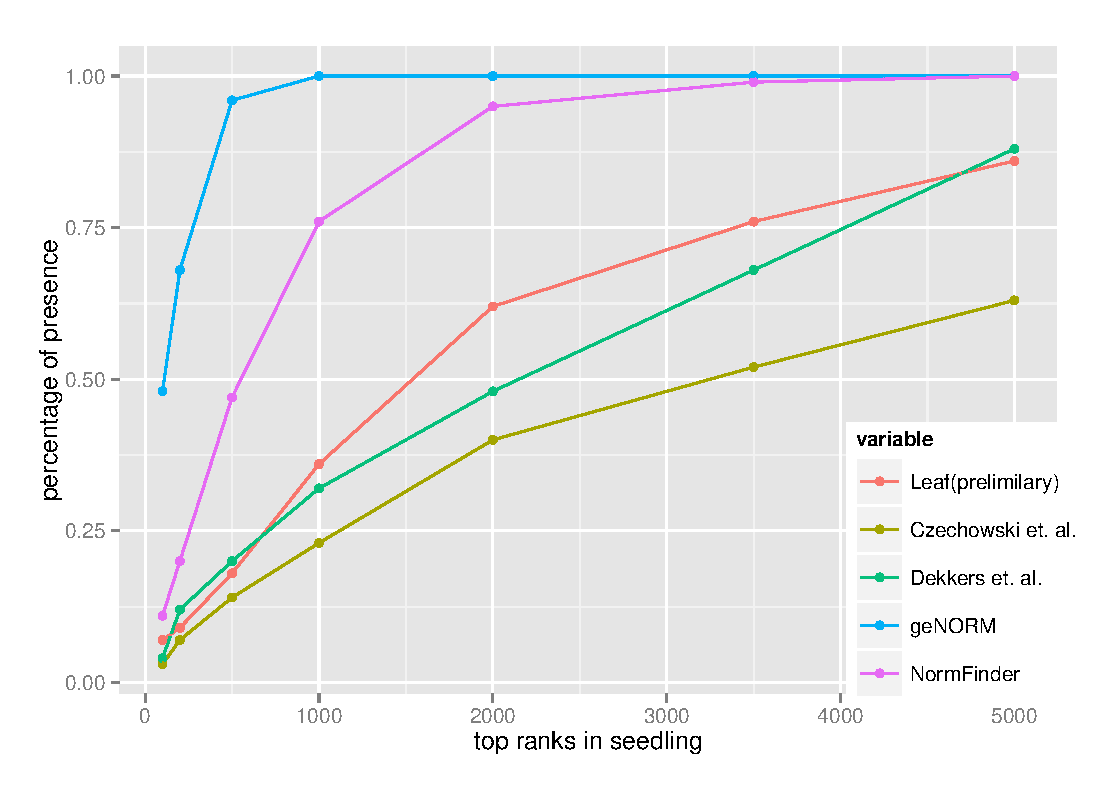
\includegraphics[scale=0.4]{Figures/C1.eps}
%\includegraphics[scale=0.4]{Figures/C2.eps}
%\includegraphics[scale=0.4]{Figures/C3.eps}
%\caption{{\small{\label{sup:expressinlevel} expression levels of Arabidopsis RNA-Seq leaf data: traditional reference genes in set 3 (top)};  5 stably expressed genes by  Czechowski et. al. (middle); 5 stably expressed genes identified by total variance (bottom)}}
%\end{center}
%\end{figure} 


% \begin{figure}[h!]
%\begin{center}
%\includegraphics[scale=0.5]{./Figures/rank_sl.eps}
%\includegraphics[scale=0.5]{./Figures/rank_st.eps}
%\caption{\label{fig:rankAgainstrank} Rank plot of stably expressed genes,  Set 1 versus Set 2 and Set 3.}
%\end{center}
%\end{figure}
%
% \begin{figure}[h!]
%\begin{center}
%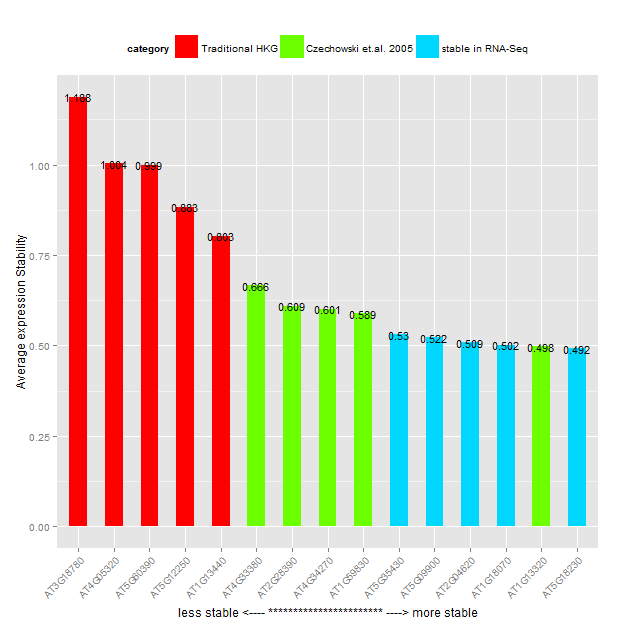
\includegraphics[scale=0.3]{Figures/mvalue2.eps}
%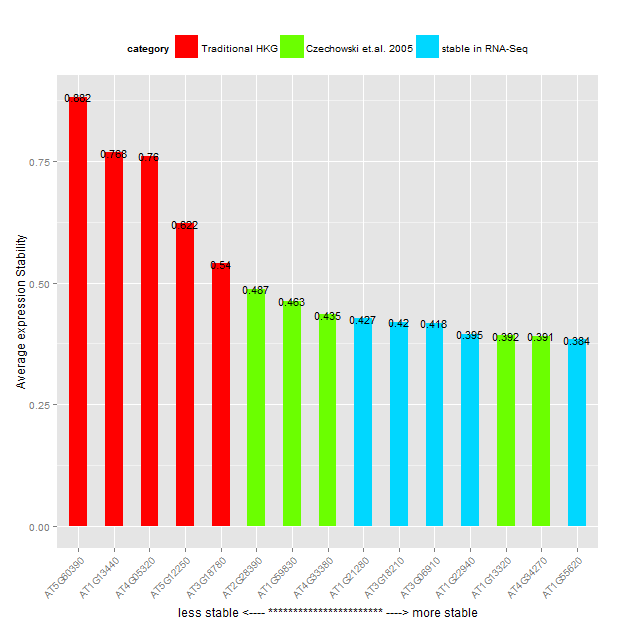
\includegraphics[scale=0.3]{Figures/mvalue3.eps}
%\caption{\label{sup:mvalue} geNORM ranking of reference genes: 5 traditional HKGs, 5 reference genes identified by Czechowski et. al. and 8 stably expressed genes based on seedling RNA-Seq data.  The spearman correlations of $M$ values and total variance  are 0.989 and 0.977, respectively. }
%\end{center}
%\end{figure}


\newpage


\bibliographystyle{apalike}
\bibliography{mybib}

\end{document}

we randomly choose five genes from top 100 stably expressed genes identified from leaves group, and compared them to five genes randomly chosen from top 100 stably expressed genes of multiple-tissue group. Figure \ref{expressinlevel2} displays the expression profiles in CPM over the five experiments in leaves group. Three genes from multiple-tissue group show large between-experiment variation in leaves group. As we commented earlier, genes that are stable under a wider range of conditions may not be the most stable ones under a narrow set of conditions.



\begin{figure}
\centering
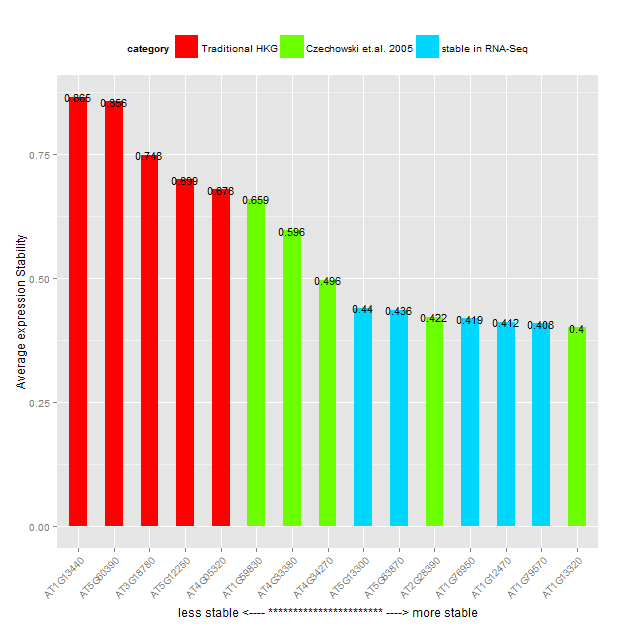
\includegraphics[width=0.7\linewidth]{Figures/mvalue1}
\caption{}
\label{fig:mvalue1}
\end{figure}



 \begin{figure}[H]
 \begin{center}
	%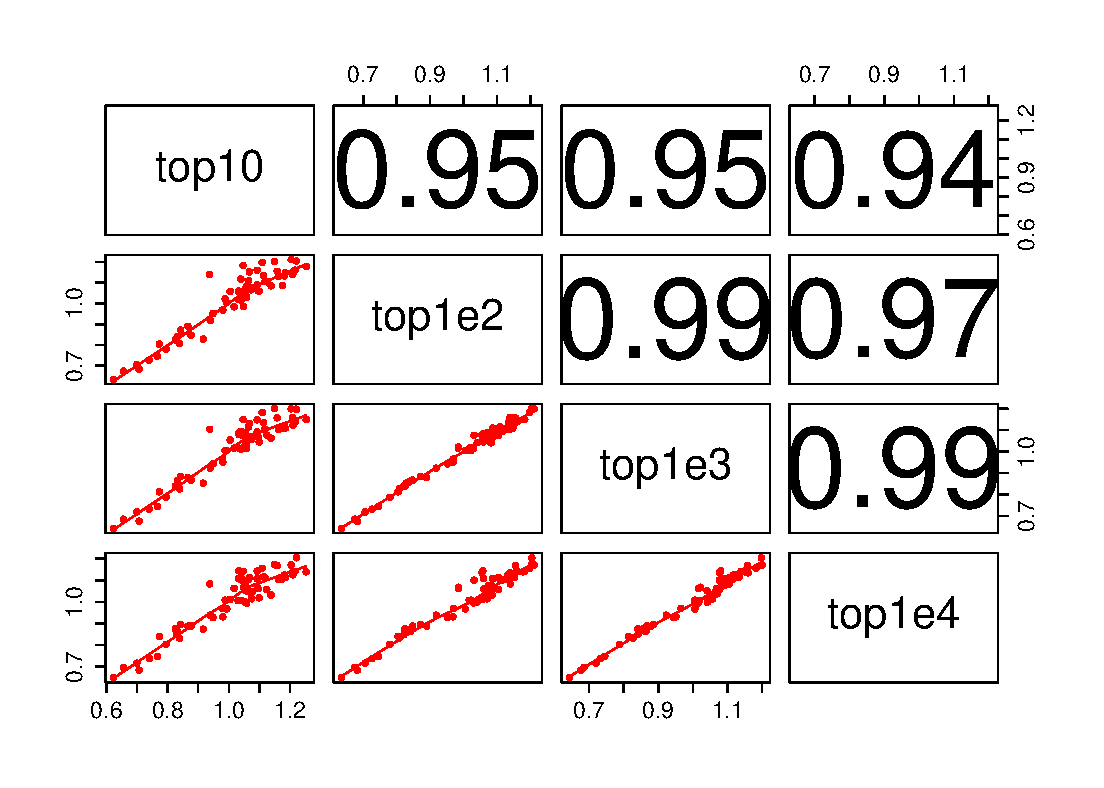
\includegraphics[scale=0.5]{Figures/B1.eps}
	
	\includegraphics[scale=0.4][Figures/tissue_leaf.eps}
	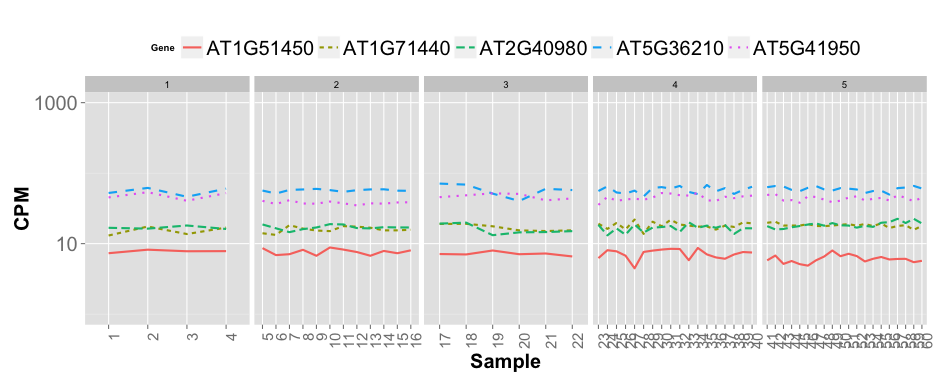
\includegraphics[scale=0.4]{Figures/leaf_leaf.eps}
	\caption{{\small{\label{expressinlevel2} Expression levels CPM plotted using leaves data: 5 stably expressed genes randomly selected from top 100 of leaves group (top) ; 5 stably expressed genes randomly selected from top 100 of multiple-tissue group }}}
\end{center}
\end{figure} 


